\chapter{Криптографические протоколы}\index{протокол!криптографический}\label{chapter-protocols}
\selectlanguage{russian}

% Протокол без разрывов между страницами, но зато
% разрешаем разрывать страницу до и после определения протокола
% (по умолчанию itemize / enumerate так не разрешают)
\newsavebox{\protocolbox}
\makeatletter\newenvironment{protocol}{%
\begin{samepage}%
\@beginparpenalty=\@lowpenalty%
\@endparpenalty=\@lowpenalty%
\begin{itemize}}
{\end{itemize}\end{samepage}}\makeatother
% Разрешить разрывать страницу для длинных протоколов
\makeatletter\newenvironment{protocol*}{%
\begin{itemize}}
{\end{itemize}}\makeatother

% https://tex.stackexchange.com/questions/164707/how-to-use-greek-letters-in-pgf-umlsd-or-generally-terms-starting-with
\renewcommand{\mess}[4][0]{
	\stepcounter{seqlevel}
	\path
	(#2)+(0,-\theseqlevel*\unitfactor-0.7*\unitfactor) node (mess from) {};
	\addtocounter{seqlevel}{#1}
	\path
	(#4)+(0,-\theseqlevel*\unitfactor-0.7*\unitfactor) node (mess to) {};
	\draw[->,>=angle 60] (mess from) -- (mess to) node[midway, above]
	{#3};

	\node (\detokenize{#3} from) at (mess from) {};
	\node (\detokenize{#3} to) at (mess to) {};
}


\chapter{Основные понятия и определения}
\selectlanguage{russian}

Изучение курса <<Защита информации>> необходимо начать с определения понятия \emph{<<информация>>}. В теоретической информатике \emph{информация} -- это любые сведения, или цифровые данные, или сообщения, или документы, или файлы, которые могут быть переданы \emph{получателю информации} от \emph{источника информации}. Можно считать, что информация передаётся по какому-либо каналу связи с помощью некоторого носителя, которым может быть, например, распечатка текста, диск или другое устройство хранения информации, система передачи сигналов по оптическим, проводным линиям или радиолиниям связи и~т.\,д.

\emph{Защита информации} -- это сохранение \emph{целостности}, \emph{конфиденциальности} и \emph{доступности} информации, передаваемой или хранимой в какой-либо форме. Информацию необходимо защищать от разрушения её целостности и конфиденциальности в результате вмешательства \emph{нелегального пользователя}. В российском стандарте ГОСТ Р 50.1.056-2005 приведены следующие определения~\cite{GOST-2005}:
\begin{itemize}
	\item \emph{целостность информации}\index{целостность} -- состояние информации, при котором отсутствует любое ее изменение либо изменение осуществляется только преднамеренно субъектами, имеющими на него право;
	\item \emph{конфиденциальность}\index{конфиденциальность} -- состояние информации, при котором доступ к ней осуществляют только субъекты, имеющие на него право;
	\item \emph{доступность}\index{доступность} -- состояние информации, при котором субъекты, имеющие права доступа, могут реализовать их беспрепятственно.
\end{itemize}

Чтобы реализовать защиту информации, используются различные математические методы, технические средства и организационные меры. В частности, источник информации (на передающей стороне) применяет \emph{шифрование}, а легальный пользователь (на приёмной стороне) осуществляет \emph{расшифрование}\index{расшифрование}. Процесс получения информации нелегальным пользователем называется \emph{дешифрованием}\index{дешифрование}\footnote{В англоязычной литературе словом <<decryption>> обозначается и расшифрование, и дешифрование.}, а сам нелегальный пользователь -- \emph{криптоаналитиком}\index{криптоаналитик}.

\section{Модель системы передачи с криптозащитой}
\selectlanguage{russian}

Простая модель системы передачи с криптозащитой представлена на рис.~\ref{pic:Encrypt}, где введены следующие обозначения:
\begin{itemize}
    \item $A$ -- источник информации;
    \item $B$ -- получатель информации, легальный пользователь;
    \item $X$ -- сообщение до шифрования или \emph{открытый текст}\index{открытый текст} (\langen{plaintext}); $\set{M}$ -- множество всех возможных открытых текстов (от слова Message), $X \in \set{M}$;
    \item $K_1$ -- ключ шифрования\index{ключ!шифрования} (\langen{encryption key}); $\set{K}_E$ -- множество всех возможных ключей шифрования, $K_1 \in \set{K}_E$;
    \item $Y$ -- зашифрованное сообщение (\emph{шифротекст}\index{шифротекст}, \langen{ciphertext, cyphertext} или \emph{шифрограмма}\index{шифрограмма}\footnote{Строго говоря, \emph{шифрограмма} -- это \emph{шифротекст} после его \emph{кодирования} для целей передачи по каналу связи}); $\set{C}$ -- множество всех возможных шифротекстов, $Y \in \set{C}$;
    \item $K_2$ -- ключ расшифрования\index{ключ!расшифрования} (\langen{decryption key}); $\set{K}_D$  -- множество возможных ключей расшифрования, зависящее от множества $\set{K}_E$, $K_2 \in \set{K}_D$.
\end{itemize}

\begin{figure}[!thb]
	\centering
	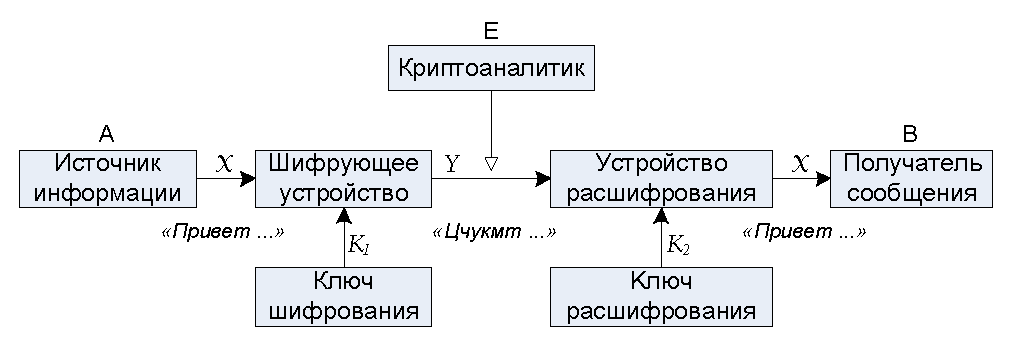
\includegraphics[width=1.0\textwidth]{pic/scheme-of-cipher}
	\caption{Передача информации с криптозащитой\label{pic:Encrypt}}
\end{figure}

\emph{Шифр}\index{шифр} -- это множество обратимых функций отображения $E_{K_1}$\index{функция!шифрования} множества открытых текстов $\set{M}$ на множество шифротекстов $\set{C}$, зависящих от выбранного ключа шифрования $K_1$ из множества $\set{K}_E$:
%обратимое отображение пары из элемента множества открытых текстов $\set{M}$ и элемента множества ключей шифрования $\set{K}_E$ в множество шифротекстов $\set{C}$:
\begin{equation}
    \label{eq:Encryption}
    Y = E_{K_1}(X), ~ X \in \set{M}, ~ K_1 \in \set{K}_E, ~ Y \in \set{C}.
\end{equation}
Можно сказать, что шифрование -- это обратимая функция двух аргументов: сообщения и ключа. Для каждого $K_1$ эта функция должна быть обратимой. Обратимость -- основное условие шифрования, по которому каждому зашифрованному сообщению $Y$ и ключу $K$ соответствует одно исходное сообщение $X$. Легальный пользователь $B$ (на приемной стороне системы связи)  получает сообщение $Y$ и осуществляет процедуру \emph{расшифрования}\index{расшифрование}.
Следует отличать шифрование от кодирования, так как кодирование -- это процесс сопоставления конкретным сообщениям строго определенной комбинации символов или сигналов, с целью повышения помехоустойчивости передаваемого сигнала.
Расшифрование --  это отображение множества шифротекстов $\set{C}$ на множество открытых текстов $\set{M}$ функцией $D_{K_2}$\index{функция!расшифрования}, зависящей от ключа расшифрования $K_2$ из множества $\set{K}_D$, являющейся обратной к функции $E_{K_1}$.
\begin{equation}
    \label{eq:Decryption}
    D_{K_2}(Y) = X, ~ Y \in \set{C}, ~ K_2 \in \set{K}_D, ~ X \in \set{M}.
\end{equation}

%Система передачи информации с криптозащитой называется \emph{криптосистемой}\index{криптосистема}.(?????)

%В общем случае функция шифрования сюръективна и псевдослучайна, отображая один открытый текст в разные шифротексты. Если функция шифрования биективна, на практике ее инкапсулируют в другую функцию с целью добиться псевдослучайности шифрования одинаковых открытых текстов в разные шифротексты.

%Методы защиты информации зависят от возможных сценариев передачи. Рассмотрим несколько основных вариантов.
Рассмотрим возможные сценарии вмешательства криптоаналитика и организации защиты информации от его действий.
Пусть  $A$ --  источник и $B$ -- получатель сообщений.

\begin{description}
    \item[Сценарий 1.] Пусть $E$ -- \emph{пассивный} криптоаналитик\index{криптоаналитик!пассивный}, который может подслушивать передачу, но не может вмешиваться в процесс передачи. Из пассивности криптоаналитика следует, что $Y = \widetilde{Y}$, и \emph{целостность} информации обеспечена.

Цель защиты --- \emph{обеспечение конфиденциальности}.

Средства защиты -- шифрование с помощью \emph{симметричных} или \emph{асимметричных } криптосистем.

Дополнительные задачи -- при большом числе пользователей должна быть решена задача \emph{генерации и доставки секретных ключей} всем пользователям.

    \item[Сценарий 2.] Пусть $E$ -- \emph{активный} криптоаналитик\index{криптоаналитик!активный}, который может изменять, удалять и вставлять сообщения или их части.

    Цель защиты -- \emph{обеспечение конфиденциальности} и  \emph{обеспечение целостности}.

Средства защиты --  шифрование и добавление \emph{имитовставки}\index{имитовставка} (message authentication code -- $\MAC$), позволяющего обнаружить нарушение целостности.

    \item[Сценарий 3.] Пусть $E$ -- активный криптоаналитик, который может изменять, удалять и вставлять сообщения или их части, дополнительно к этому легальные пользователи $A$ и $B$ не доверяют друг другу.

Цель защиты -- \emph{аутентификация} пользователей и документов.

Средства -- \emph{электронная подпись} и протокол идентификации (аутентификации) пользователей.
\end{description}

%%Возможно вмешательство нелегального пользователя $E$, называемого \emph{криптоаналитиком}.
%%
%%
%%Если $X = \widetilde{X}$, то вмешательство криптоаналитика  $E$ не изменило передаваемое сообщение, и \emph{целостность} информации обеспечена. Если криптоаналитик не получил информацию, содержащуюся в сообщении, то обеспечена \emph{конфиденциальность}.
%%
%%Если в этой системе возможна двусторонняя передача, то есть от $A$ к $B$ и от $B$ к $A$, то говорят о взаимном обмене информацией между легальными пользователями.
%
%Секретность информации в современных шифрах обеспечивается секретным ключом, в то время как сам алгоритм криптосистемы является общеизвестным. Исторический опыт, например, система шифрования A5/1 в GSM, показывает, что секретность алгоритма шифрования \emph{ослабляет} криптостойкость шифра, а не увеличивает, из-за того, что система становится малоизученной.


\section{Классификация криптосистем}

\subsection{Симметричные и асимметричные криптосистемы}
\selectlanguage{russian}

Криптографические системы и шифры можно разделить на две больших группы, в зависимости от принципа использования ключей для шифрования и расшифрования.

Если для шифрования и расшифрования используется один и тот же ключ $K$, либо если получение ключа расшифрования $K_2$ из ключа шифрования $K_1$ является тривиальной операцией, то такая криптосистема называется \textbf{симметричной}\index{криптосистема!симметричная}. В зависимости от объёма обработки данных за одну операцию шифрования симметричные шифры делятся на \textbf{блочные}\index{шифр!блочный}, в которых за одну операцию шифрования происходит преобразование одного блока данных (32 бита, 64, 128 или больше) и \textbf{потоковые}\index{шифр!потоковый}, в которых работают с каждым символом открытого текста по отдельности (например, с 1 битом или 1 байтом). Примеры блочных шифров рассмотрены в главе~\ref{chapter-block-ciphers}, а потоковых -- в главе~\ref{chapter-stream-ciphers}.

Шифрование блочным шифром подразумевает разделение открытого текста на блоки одинаковой длины. Блоки шифруются последовательно, причём результат шифрования следующего блока может зависеть от предыдущего. Это регулируется \textbf{режимом сцепления блоков}. Примеры нескольких таких режимов рассмотрены в разделе~\ref{chapter-block-chaining}.

Если ключ расшифрования получить из ключа шифрования сложно (или невозможно), то такие криптосистемы называют криптосистемами \textbf{с открытым ключом}\index{криптосистема!с открытым ключом} или \textbf{асимметричными} криптосистемами\index{криптосистема!асимметричная}. Некоторые из них рассмотрены в главе~\ref{chapter-public-key}. Все используемые на сегодняшний день асимметричные криптосистемы работают с блоком данных открытого текста, представленным в виде числа длиной в несколько сот или тысяч бит, поэтому классификация таких систем по объёму обрабатываемых за одну операцию данных не производится.

Алгоритм, который выполняет отображение аргумента произвольной длины в значение фиксированной длины, называется \textbf{хеш-функцией}. Если для такой хеш-функции выполняются определённые свойства устойчивости к поиску коллизий, то это уже \textbf{криптографическая хеш-функция}. Такие функции рассмотрены в главе~\ref{chapter-hash-functions}. Криптографические хеш-функции используются для проверки целостности сообщений. Для проверки с использованием общего секретного ключа отправителя и получателя используется механизм \textbf{имитовставки}, рассмотренный в разделе~\ref{section-MAC}. Её аналогом в криптосистемах с открытым ключом является \textbf{электронная подпись}, алгоритмы генерации и проверки которой рассмотрены в главе~\ref{chapter-public-key}, вместе с алгоритмами асимметричного шифрования.


\subsection{Шифры замены и перестановки}

Шифры по способу преобразования открытого текста в шифротекст разделяются на шифры замены и шифры перестановки.

\subsubsection{Шифры замены}
\selectlanguage{russian}

В шифрах \textbf{замены} символы одного алфавита заменяются символами другого алфавита обратимым преобразованием. В последовательности открытого текста символы входного алфавита заменяются на символы выходного алфавита. Такие шифры применяются как в симметричных системах, так и в асимметричных криптосистемах. Если при преобразовании используются однозначные функции, то шифры замены называются однозначными шифрами замены. Если используются многозначные функции, то шифры называются многозначными шифрами замены (омофонами).

В \textbf{омофоне}\index{омофон} символам входного алфавита ставится в соответствие непересекающиеся подмножества символов выходного алфавита. Количество символов в каждом подмножестве замены пропорционально частоте встречаемости символа открытого текста. Таким образом, омофон создает равномерное распределение символов шифротекста и прямой частотный криптоанализ не возможен. При шифровании омофонами символ входного алфавита заменяется на случайно выбранный из подмножества замены.

Шифры бывают \textbf{моноалфавитные}, когда для шифрования используется одно отображение входного алфавита в выходной алфавит. Если алфавит на входе и выходе одинаков и его размер (число символов) равен $D$, тогда количество всевозможных моноалфавитных шифров замены такого типа равно $D!$.

\textbf{Полиалфавитный} шифр задается множеством различных вариантов отображения входного алфавита на выходной алфавит. Шифры замены могут быть как потоковыми, так и блоковыми. Однозначный полиалфавитный потоковый шифр замены называется \textbf{шифром гаммирования}\index{шифр!гаммирования}. Символом алфавита может быть, например, 256-битовое слово, а размер алфавита -- $2^{256}$, соответственно.


\subsubsection{Шифры перестановки}

Шифры \textbf{перестановки} реализуются следующим образом. Берут открытый текст, например буквенный, и разделяют на блоки  определенной длины $x_1, x_2, \dots, x_m$. Затем осуществляется перестановка позиций блока (вместе с символами). Перестановки могут быть однократные и многократные. Частный случай перестановки -- сдвиг. Приведем пример:
\begin{center}
    секрет $\xrightarrow{\text{сдвиг}}$ ретсек $\xrightarrow{\text{перестановка}}$ рскете.
\end{center}
Ключ такого шифра указывает  изменение порядка номеров  позиций блока  при  шифровании и  расшифровании.

Существуют так называемые \textbf{маршрутные перестановки}. Используется какая-либо геометрическая фигура, например, прямоугольник. Запись открытого текста ведется по одному \emph{маршруту}, например по строкам, а считывание для шифрования осуществляется по другому маршруту, например по столбцам. Ключ шифра определяет эти маршруты.
В случае, когда рассматривается перестановка блока текста фиксированной длины, перестановку можно рассматривать как замену.

В полиалфавитных шифрах при шифровании открытый текст разбивается на блоки (последовательности) длины $n$, где $n$ -- \textbf{период}. Этот параметр выбирает \emph{криптограф} и держит его в секрете.

Поясним процедуру шифрования полиалфавитным шифром. Запишем шифруемое сообщение  в  матрицу по столбцам определенной длины. Пусть открытый текст таков: <<Игры различаются по содержанию, характерным особенностям, а также по тому, какое место они занимают в жизни детей>>. Зададим $n=4$ и запишем этот текст в  матрицу размера $(4 \times 24)$:

\begin{center} \resizebox{\textwidth}{!}{ \begin{tabular}{|c|c|c|c|c|c|c|c|c|c|c|c|c|c|c|c|c|c|c|c|c|c|c|c|}
    \hline
    и&р&и&т&о&е&н&а&т&ы&о&н&я&а&п&м&к&е&о&а&а&ж&и&е \\
    г&а&ч&с&с&р&и&р&е&м&б&о&м&к&о&у&о&с&н&н&ю&и&д&й \\
    р&з&а&о&ж&р&ю&а&р&о&е&с&а&ж&т&к&е&т&и&и&т&з&е& \\
    ы&л&ю&п&д&а&х&к&н&с&н&т&т&е&о&а&м&о&з&м&в&н&т& \\
    \hline
\end{tabular} } \end{center}

Выбираем $4$ различных моноалфавитных шифра.

Первую строку

\begin{center} \resizebox{\textwidth}{!}{ \begin{tabular}{|c|c|c|c|c|c|c|c|c|c|c|c|c|c|c|c|c|c|c|c|c|c|c|c|}
    \hline
    и&р&и&т&о&е&н&а&т&ы&о&н&я&а&п&м&к&е&о&а&а&ж&и&е \\
    \hline
\end{tabular} } \end{center}

 шифруем, используя первый шифр. Вторую строку

\begin{center} \resizebox{\textwidth}{!}{ \begin{tabular}{|c|c|c|c|c|c|c|c|c|c|c|c|c|c|c|c|c|c|c|c|c|c|c|c|}
    \hline
    г&а&ч&с&с&р&и&р&е&м&б&о&м&к&о&у&о&с&н&н&ю&и&д&й \\
    \hline
\end{tabular} } \end{center}

шифруем, используя второй шифр, и т.д.

Выполняя расшифрование, легальный пользователь знает период. Он записывает принятую шифрограмму по строкам в матрицу с длиной строки, равной периоду, и к каждому столбцу применяет соответствующий ключ и расшифровывает сообщение, зная соответствующие шифры.

Шифры перестановки можно рассматривать как частный случай шифров замены, если отождествить один блок перестановки с одним символом большого алфавита.


\subsubsection{Композиционные шифры}
\selectlanguage{russian}

Почти все современные шифры являются \emph{композиционными}~\cite{AlZKCh:2001}. Также распространено название \emph{составные шифры}, впервые введенное в работе Клода Шеннона (\langen{Claude Elwood Shannon},~\cite{Shannon:1949:CTS}). В них применяются несколько различных методов шифрования к одному и тому же открытому тексту. В современных криптосистемах используется,например, композиция шифра замены и шифра перестановок, применяемая многократно.


\subsection{Примеры современных криптографических примитивов}

Приведём примеры названий некоторых современных криптографических примитивов, из которых строят системы защиты информации:
\begin{itemize}
    \item DES\index{шифр!DES}, AES, ГОСТ 28147-89, Blowfish\index{шифр!Blowfish}, RC5\index{шифр!RC5}, RC6\index{шифр!RC6} -- блочные симметричные шифры, скорость обработки -- десятки мегабайт в секунду;
    \item A5/1, A5/2, A5/3\index{шифр!A5}, RC4\index{шифр!RC4} -- потоковые симметричные шифры с высокой скоростью, семейство A5 применяется в мобильной связи GSM, RC4 -- в компьютерных сетях для SSL-соединения между браузером и веб-сервером;
    \item RSA\index{шифр!RSA} -- криптосистема с открытым ключом для шифрования;
    \item RSA\index{электронная подпись!RSA}, DSA\index{электронная подпись!DSA}, ГОСТ Р 34.10-2001\index{электронная подпись!ГОСТ Р 34.10-2001} -- криптосистемы с открытым ключом для электронной подписи;
    \item MD5\index{хэш-функция!MD5}, SHA-1\index{хэш-функция!SHA-1}, SHA-2\index{хэш-функция!SHA-2}, ГОСТ Р 34.11-94\index{хэш-функция!ГОСТ Р 34.11-94} -- криптографические хэш-функции.
\end{itemize}

\section{Методы криптоанализа и типы атак}
\selectlanguage{russian}

Нелегальный пользователь-криптоаналитик получает информацию путём дешифрования. Сложность этой процедуры определяется числом стандартных операций, которые надо выполнить для достижения цели. \emph{Двоичной сложностью}\index{сложность!двоичная} (или битовой сложностью) алгоритма называется количество двоичных операций, которые необходимо выполнить для его завершения.
% Наиболее сложным является дешифрование полиалфавитных шифров.

Рассмотрим основные сценарии работы криптоаналитика $E$. В первом сценарии криптоаналитик может осуществлять подслушивание и (или) перехват сообщений. Его вмешательство не нарушает целостности информации: $Y=\widetilde{Y}$. Эта роль криптоаналитика называется \emph{пассивной}. Так как он получает доступ к информации, то здесь нарушается конфиденциальность.

Во втором сценарии роль криптоаналитика \emph{активная}. Он может подслушивать, перехватывать сообщения и преобразовывать их по своему усмотрению: задерживать, искажать с помощью перестановок пакетов, устраивать обрыв связи, создавать новые сообщения и т.~п. В этом случае выполняется условие $Y \neq \widetilde{Y}$. Это значит, что одновременно нарушается целостность и конфиденциальность передаваемой информации.

Приведём примеры пассивных и активных атак:
\begin{itemize}
    \item Атака <<\emph{человек посередине}>>\index{атака!<<человек посередине>>} (\langen{man-in-the-middle}) подразумевает криптоаналитика, который разрывает канал связи, встраиваясь между $A$ и $B$, получает сообщения от $A$ и от $B$, а от себя отправляет новые, фальсифицированные сообщения. В результате $A$ и $B$ не замечают, что общаются с $E$, а не друг с другом.
    \item Атака \emph{воспроизведения}\index{атака!воспроизведения} (\langen{replay attack}) предполагает, что криптоаналитик может записывать и воспроизводить шифротексты, имитируя легального пользователя.
    \item Атака на \emph{различение} сообщений\index{атака!на различение} означает, что криптоаналитик, наблюдая одинаковые шифротексты, может извлечь информацию об идентичности исходных открытых текстов.
    \item Атака на \emph{расширение} сообщений\index{атака!на расширение} означает, что криптоаналитик может дополнить шифротекст осмысленной информацией без знания секретного ключа.
    \item \emph{Фальсификация} шифротекстов\index{атака!фальсификацией} криптоаналитиком без знания секретного ключа.
\end{itemize}

Часто для нахождения секретного ключа криптоатаки строят в предположениях о доступности дополнительной информации. Приведём примеры:
\begin{itemize}
    \item Атака на основе известного открытого текста\index{атака!с известным открытым текстом} (\langen{chosen plaintext attack, CPA}) предполагает, что криптоаналитик имеет возможность выбирать открытый текст и получать для него соответствующий шифротекст.
    \item Атака на основе известного шифротекста\index{атака!с известным шифротекстом} (\langen{chosen ciphertext attack, CCA}) предполагает возможность криптоаналитику выбирать шифротекст и получать для него соответствующий открытый текст.
\end{itemize}

Обязательным требованием к современным криптосистемам является устойчивость ко всем известным типам атак: пассивным, активным и с дополнительной информацией.


%Приведём примеры возможных вариантов работы активного криптоаналитика.
%\begin{itemize}
%\item Криптоаналитик имеет $m$ шифрованных сообщений $Y_{1},Y_{2},\ldots Y_{m}$ и пытается определить ключ или прочитать открытый текст $X_{1},X_{2},\ldots X_{m}.$
%\item Криптоаналитик имеет несколько пар открытого и шифрованного текстов
%
%$(Y_{1},X_{1}),(Y_{2}X_{2}),\ldots (Y_{m}X_{m})$ и пытается дешифровать остальной текст или определить алгоритм шифрования или определить ключ.
%\item
%\item
%\item
%\end{itemize}

Для защиты информации от активного криптоаналитика и обеспечения её целостности дополнительно к шифрованию сообщений применяют имитовставку\index{имитовставка}. Для неё используют обозначение $\MAC$ (\langen{message authentication code}). Как правило, $\MAC$ строится на основе хэш-функций, которые будут описаны далее.

Существуют ситуации, когда пользователи $A$ и $B$ не доверяют друг другу. Например, $A$ -- банк, $B$ -- получатель денег. $A$ утверждает, что деньги переведены, $B$ утверждает, что не переведены. Решение задачи аутентификации и неотрицаемости состоит в обеспечении \emph{электронной подписью}\index{электронная подпись} каждого из абонентов. Предварительно надо решить задачу о генерировании и распределении секретных ключей.

В общем случае, системы защиты информации должны обеспечивать:
\begin{itemize}
    \item конфиденциальность\index{конфиденциальность} (защита от наблюдения);
    \item целостность\index{целостность} (защита от изменения);
    \item аутентификацию (защита от фальсификации пользователя и сообщений);
    \item доказательство авторства информации (доказательство авторства и защита от его отрицания).
\end{itemize}
как со стороны получателя, так и со стороны отправителя.

Важным критерием для выбора степени защиты является сравнение стоимости реализации взлома для получения информации и экономического эффекта от владения ей. Очевидно, что если стоимость взлома превышает ценность информации, взлом нецелесообразен.

%Сценарии защиты информации
%   Сценарий 1. A -- передающая сторона. B -- принимающая сторона. E -- пассивный
%криптоаналитик, который может подслушивать передачу, но не может вмешиваться
%в процесс передачи. Цель защиты: обеспечение конфиденциальности. Средства
%-- методы шифрования с секретным ключом (симметричные системы шифрования)
%и методы шифрования с открытым ключом (асимметричные системы шифрования).
%Сценарий 2. E -- активный криптоаналитик, который может изменять, удалять и вставлять
%сообщения или их части. Цель защиты -- обеспечение конфиденциальности (не
%всегда) и обеспечение целостности. Средства -- методы шифрования и добавление
%имитовставки\index{имитовставка} (Message Autentication Code -- $\MAC$).
%Сценарий 3. A и B не доверяют друг другу. Цель защиты -- аутентификация пользователя.
%Средства -- электронная подпись.


\section{Минимальные длины ключей}
\selectlanguage{russian}

Оценим минимальную битовую длину ключа для обеспечения криптостойкости, то есть защиты криптосистемы от атаки, полным перебором всех возможных секретных ключей. Сделаем такие предположения:

\begin{itemize}
    \item одно ядро процессора выполняет $R = 10^7 \approx 2^{23}$ шифрований и расшифрований в секунду;
    \item вычислительная сеть состоит из $n = 10^3 \approx 2^{10}$ узлов;
    \item в каждом узле имеется $C = 16 = 2^4$ ядер процессора;
    \item нужно обеспечить защиту данных на $Y = 100$ лет, т.е. на $S \approx 2^{32}$ с;
    \item выполняется закон Мура об удвоении вычислительной производительности на единицу стоимости каждые 2 года, то есть производительность вырастет в $M = 2^{Y/2} \approx 2^{50}$ раз.
\end{itemize}

Число переборов $N$ примерно равно
    \[ N \approx R \cdot n \cdot C \cdot S \cdot M, \]
    \[ N \approx 2^{23} \cdot 2^{10} \cdot 2^{4} \cdot 2^{32} \cdot 2^{50} = 2^{23+10+4+32+50} = 2^{119}. \]

Следовательно, минимально допустимая длина ключа для защиты от атаки перебором на 100 лет составляет порядка
    \[ \log_2 N \approx 119\text{ бит} \] .

Например, в 1997 году предыдущий американский стандарт шифрования DES с 56-битовым секретным ключом впервые был взломан перебором интернет-сетью из 78 000 частных компьютеров, производивших фоновые вычисления по проекту \textsc{DesChal}.



\input{writing-rules}

\section{Свойства безопасности протоколов}
\selectlanguage{russian}
Защищённая система и, соответственно, защищённый протокол могут выполнять разные функции безопасности. Многие из этих функций или целей (\langen{{goals}}) можно сформулировать как устойчивость к определённому классу атак. Наиболее полным и актуальным считается перечисление и толкование этих целей в документе проекта AVISPA (\langen{Automated Validation of Internet Security Protocols and Applications})~\cite{AVISPA:2003}, суммирующим описания из различных документов IETF (\langen{{Internet Engineering Task Force}}). Данные цели принято считать \emph{формализируемыми} -- то есть такими, что для отдельных протоколов есть возможность формально доказать или опровергнуть достижение этих целей.

\begin{itemize}
	\item Аутентификация (однонаправленная).\\*
		\langen{Authentication (unicast)}.
	\begin{itemize}
		\item[(G1)] Аутентификация субъекта.\\*
			\langen{Entity authentication (Peer Entity Authentication)}.
		\item[{}] Гарантия для одной стороны протокола через представление доказательств и / или учётных данных второй стороны, участвующей в протоколе, и того, что вторая сторона действительно участвовала в текущем сеанса протокола. Обычно делается через представления таких данных, которые могли быть сгенерированы только второй стороной. Аутентификация субъекта подразумевает, что полученные данные могут быть однозначно прослежены до субъекта протокола, что подразумевает аутентификацию источника данных.
		\item[(G2)] Аутентификация сообщения.\\*
			\langen{Message authentication (Data Origin Authentication)}.
		\item[{}] Гарантия того, что полученное сообщение или фрагмент данных были созданы определённым субъектом в какое-то (обычно неуказанное) время в прошлом, и что эти данные не были повреждены или подделаны. Но без предоставления уникальности или своевременности. Аутентификация сообщений подразумевает их целостность.
		\item[(G3)] Защита от повтора.\\*
			\langen{Replay Protection}.
		\item[{}] Защита от ситуации, когда некоторая сторона запишет некоторое сообщение и воспроизведёт его позднее (возможно -- в другом сеансе протокола), что приведёт к некорректной интерпретации данной стороны как аутентифицированной.
	\end{itemize}

	\item Аутентификация при рассылке по многим адресам или при подключении к службе подписки/уведомления.\\*
		\langen{Authentication in Multicast or via a Subscribe / Notify Service}.
	\begin{itemize}
		\item[(G4)] Явная аутентификация получателя.\\*
			\langen{Implicit Destination Authentication}.
		\item[{}] Протокол должен гарантировать, что отправленное сообщение доступно для чтения только легальным получателям. То есть только легальные авторизованные участники будут иметь доступ к актуальной информации, многоадресному сообщению или сеансу групповой связи. Включает в себя группы рассылки с очень динамичным членством.
		\item[(G5)] Аутентификация источника.\\*
			\langen{Source Authentication}.
		\item[{}] Легальные получатели смогут аутентифицировать источник и содержание информации или группового общения. Включает случаи, когда члены группы не доверяют друг другу.
	\end{itemize}

	\item[(G6)] Авторизация (третьей доверенной стороной).\\*
		\langen{Authorization (by a Trusted Third Party)}.
	\item[{}] Гарантия возможности авторизовать (в терминах протокола) одного субъекта на доступ к ресурсу другого с помощью третьей доверенной стороны. Подразумевает, что владелец ресурса может не иметь собственных списков доступа (\langen{Access Control List, ACL})) и полагается на таковые у доверенной стороны.

	\item Совместная генерация ключа.\\*
		\langen{Key Agreement Properties}.
	\begin{itemize}
		\item[(G7)] Аутентификация ключа.\\*
			\langen{Key authentication}.
		\item[{}] Гарантия для одного из субъектов, что только легальные пользователи могут получить доступ к конкретному секретному ключу.
		\item[(G8)] Подтверждение владения ключом.\\*
			\langen{Key confirmation (Key Proof of Possession)}.
		\item[{}] Гарантия для одного из субъектов, что другой субъект действительно владеет конкретным секретным ключом (либо информацией, необходимой для получения такого ключа).
		\item[(G9)] Совершенная прямая секретность.\\*
			\langen{Perfect Forward Secrecy (PFS)}.
		\item[{}] Гарантия того, что компрометация мастер-ключей в будущем не приведёт к компрометации сессионных ключей уже прошедших сеансов протокола.
		\item[(G10)] Формирование новых ключей.\\*
			\langen{Fresh Key Derivation}.
		\item[{}] Гарантия возможности создать новые сессионные ключи для каждого сеанса протокола. 
		\item[(G11)] Защищённая возможность договориться о параметрах безопасности.\\*
			\langen{Secure capabilities negotiation (Resistance against Downgrading and Negotiation Attacks)}.
		\item[{}] Гарантия не только того, что легальные стороны имеют возможность договориться о параметрах безопасности, но и того, что нелегальная сторона не вмешалась в протокол и не привела к выбору предпочтительных ей (возможно -- наиболее слабых) параметров безопасности.
	\end{itemize}

	\item[(G12)] Конфиденциальность (секретность).\\*
		\langen{Confidentiality (Secrecy)}.
	\item[{}] Гарантия, что конкретный элемент данных (часть передаваемого сообщения) остаётся неизвестным для злоумышленника. В данной цели не рассматривается секретность сеансового ключа, проверка подлинности ключа или надёжность долговременных мастер-ключей.

	\item Анонимность.\\*
		\langen{Anonymity}.
	\begin{itemize}
		\item[(G13)] Защита идентификаторов от прослушивания (несвязываемость).\\*
			\langen{Identity Protection against Eavesdroppers}.
		\item[{}] Гарантия, что злоумышленник (подслушивающий) не состоянии связать обмен сообщениями субъектом с его реальной личностью.
		\item[(G14)] Защита идентификаторов от других участников.\\*
			\langen{Identity Protection against Peer}.
		\item[{}] Гарантия, что участник переписки не в состоянии связать обмен сообщениями субъекта с реальной личностью, но только с некоторым псевдонимом.
	\end{itemize}

	\item[(G15)] Ограниченная защита от атак отказа в обслуживании.\\*
		\langen{(Limited) Denial-of-Service (DoS) Resistance}.
	\item[{}] Гарантия, что протокол следует определённым принципам, уменьшающих вероятность (усложняющих использование) отдельных классов атак отказа в обслуживании.

	\item[(G16)] Неизменность отправителя.\\*
		\langen{Sender Invariance}.
	\item[{}] Гарантия для одной из сторон, что источник сообщения остался таким же, как тот, который начал общение, хотя фактическая идентификация источника не важна для получателя.

	\item Неотрекаемость.\\*
		\langen{Non-repudiation}.
	\begin{itemize}
		\item[(G17)] Подотчётность.\\*
			\langen{Accountability}.
		\item[{}] Гарантия возможности отслеживания действий субъектов над объектами.
		\item[(G18)] Доказательство происхождения.\\*
			\langen{Proof of Origin}.
		\item[{}] Гарантия неопровержимости доказательств источника сообщения.
		\item[(G19)] Доказательство доставки.\\*
			\langen{Proof of Delivery}.
		\item[{}] Гарантия неопровержимости доказательств факта получения сообщения.
	\end{itemize}

	\item[(G20)] Защищённое временное свойство.\\*
		\langen{Safety Temporal Property}.
	\item[{}] Гарантия возможности доказать, что факт нахождения системы в одном из состояний означает, что некогда в прошлом система хотя бы раз находилась в некотором другом состоянии. Например, что получение субъектом доступа к ресурсу означает, что некогда в прошлом субъект успешно оплатил данный доступ.

\end{itemize}

Примеры свойств безопасности, реализуемыми различными протоколами приведены в таблице~\ref{tab:protocols-properties}).

\begin{landscape}
{\renewcommand{\arraystretch}{1.5}
\begin{table}
    \centering
    \begin{tabular}{|l|c|c|c|c|c|c|c|c|c|c|c|c|c|c|c|}
        \hline
Протокол \textbackslash Цель G & 1 & 2 & 3 & 4 & 5 & 6 & 7 & 8 & 9 & 10 & 11 & 12 & 13 & 14 & 15 \\
        \hline
        EAP-IKEv2              & × & × & × &   &   & × & × &   &   &  × &    &    &    &    &  × \\
        \hline
        EKE                    & × & × &   &   &   &   &   &   &   &    &    &  × &    &    &    \\
        \hline
        IKE                    & × & × & × &   &   &   & × &   & × &  × &  × &    &  × &  × &  × \\
        \hline
        IKEv2                  & × & × & × &   &   &   & × &   & × &  × &  × &    &    &    &  × \\
        \hline
        DHCP-IPSec-tunnel      & × & × &   &   &   &   &   &   &   &    &    &  × &    &    &    \\
        \hline
        kerberos               & × & × & × &   &   & × & × &   &   &  × &    &    &    &    &    \\
        \hline
        SSH                    & × & × & × &   &   &   & × &   &   &  × &  × &    &    &    &    \\
        \hline
        TLS, TLS 1.1, TLS 1.2  & × & × & × &   &   &   & × &   &   &  × &  × &    &  × &    &    \\
        \hline
        TLS 1.3                & × & × & × &   &   &   & × &   & × &  × &  × &    &  × &    &    \\
        \hline
        SET                    & × & × & × &   &   &   &   &   &   &    &    &    &  × &    &    \\
        \hline
    \end{tabular}
    \caption{Примеры свойств безопасности протоколов (по \cite{Cheremushkin:2009} с дополнениями).}
    \label{tab:protocols-properties}
\end{table}
}
\end{landscape}


\input{classification}

\section{Атаки на протоколы}\label{section-protocols-attacks}
\selectlanguage{russian}

Защищённые свойства протоколов могут быть заявленными, когда о них заявляют сами авторы протокола (и, обычно, приводят различные аргументы в пользу выполнения данных функций), и подразумеваемыми, когда авторы некоторой системы рассчитывают на реализацию защищённых свойств некоторым протоколом.

Под \emph{атакой на защищённый протокол}\index{атака!на протокол} понимается попытка проведения анализа сообщений протокола и/или выполнения непредусмотренных протоколом действий для нарушения заявленных или подразумеваемых свойств протокола.\footnote{Используется модифицированное определение из~\cite{Cheremushkin:2009}. Отличие в том, что Черёмушкин в своём определении не описывает, что такое <<нарушение работы протокола>> и оставляет двусмысленными случаи нарушения, например, свойств G9/PFS и G20/STP.}

Атака считается \emph{успешной}, если нарушено хотя бы одно из заявленных или подразумеваемых свойств протокола.

В случае успешной атаки на подразумеваемые свойства будем уточнять, что успешна \emph{атака на использование протокола} в некоторой системе. Это будет говорить, разумеется, не о недостатках самого протокола, но о неверном выборе протокола (или его настроек) авторами системы.

Существует большое количество типов атак на протоколы. У многих атак есть некоторые общие принципы, что позволяет выделить классы атак для упрощения анализа и разработки протоколов, устойчивых к целым классам атак.

\begin{itemize}
    \item[MitM] <<Атака посередине>>\\*
        \langen{man-in-the-middle attack}
    \item[{}] Класс атак, в котором злоумышленник ретранслирует и, при необходимости, изменяет все сообщения, проходящие между двумя и более участниками протокола, причём последние не знают о существовании злоумышленника, считая, что общаются непосредственно друг с другом. К данной атаке уязвимы все протоколы, которые не реализуют взаимную аутентификацию сторон (цель G1). Классическим примером атаки данного класса является атака на протокол Диффи~---~Хеллмана\index{протокол!Диффи~---~Хеллмана}, рассмотренном в разделе~\ref{section-protocols-diffie-hellman}.

    \item[Replay] Атака с повторной передачей\\*
        \langen{replay attack}
    \item[{}] Класс атак, в котором злоумышленник записывает все сообщения, проходящие в одном сеансе протокола, а далее повторяет их в новом, выдавая себя за одного из участников первого сеанса. Примерами протоколов, к которым применима данная атака, являются протоколы Ву~---~Лама\index{протокол!Ву~---~Лама} и бесключевой протокол Шамира\index{протокол!Шамира бесключевой} из раздела~\ref{section-protocols-shamir}.

    \item[TF] Атака подмены типа\\*
        \langen{type flaw attack}
    \item[{}] Класс атак, в котором злоумышленник используя переданное в легальном сеансе протокола сообщение конструирует новое, передавая его на другом проходе (раунде) протокола под видом сообщения другого типа (с другим предназначением). К таким атакам уязвимы, например, протоколы Wide-Mouth Frog\index{протокол!Wide-Mouth Frog} из раздела~\ref{section-protocols-wide-moth-frog}, Деннинга~---~Сакко\index{протокол!Деннинга~---~Сакко}, Отвей~---~Рииса\index{протокол!Отвей~---~Рииса}, а также некоторые варианты протокола Yahalom\index{протокол!Yahalom}.

    \item[PS] Атака с параллельными сеансами\\*
        \langen{parallel-session attack}
    \item[{}] Класс атак, в котором злоумышленник инициирует несколько одновременных сеансов протокола с целью использования сообщений из одного сеанса в другом. Примером протокола, уязвимого к данному классу атак, является симметричный вариант протокола Нидхема~---~Шрёдера\index{протокол!Нидхема~---~Шрёдера}, рассмотренном в разделе~\ref{section-protocols-needham-schroeder}.

    \item[STS] Атака с известным разовым ключом\index{атака!с известным разовым ключом}\\*
        \langen{short-term secret attack}
    \item[KN] Атака с известным сеансовым ключом\\*
        \langen{known-key attack}
    \item[{}] Классы атак, в которых злоумышленник получает доступ к временным секретам, используемых в протоколах (например, новым сеансовым ключам), после чего может обеспечить, например, аутентификацию или хотя бы установление сессии от имени одной из сторон протокола.

    \item[UKS] Атака с неизвестным сеансовым ключом\\*
        \langen{unknown key-share attack}
    \item[{}] Класс атак на протоколы с аутентификацией ключа, в которых злоумышленник получает возможность доказать одной из сторон владение ключом (с помощью, например, повтора сообщения из легального сеанса), хотя сам ключ злоумышленник не знает. К такому классу атак уязвим, например, симметричный протокол Нидхема-Шрёдера из раздела~\ref{section-protocols-needham-schroeder}.

\end{itemize}

Важно отметить, что если не сказано иное, то в рамках анализа криптографических протоколов (не конкретных систем) используется предположение о стойкости всех используемых криптографических примитивов. Например, предполагается, что пока идёт защищённый обмен информацией, использующий сеансовый ключ, выработанный в сеансе некоторого криптографического протокола, то злоумышленнику не хватит ресурсов и времени на то, чтобы получить данный сеансовый ключ через атаку на используемые шифры или криптографически-стойкие хеш-функции.

С другой стороны, следует предполагать, что сеансовые ключи, получаемые в рамках сеансов протоколов, через некоторое время (однако, много большее времени самого сеанса связи) будут получены злоумышленником (классы атак STS и KN). Много позднее, возможно, злоумышленник сможет получить доступ и к <<мастер>>-ключам длительного использования, так что протоколы с генерацией сеансовых ключей должны разрабатываться в том числе со свойством G9/PFS.


\chapter{Распространение ключей}\label{chapter-key-distribution-protocols}

Задача распространения ключей является одной из множества задач построения надёжной сети общения многих абонентов. Задача состоит в получении в нужный момент времени двумя легальными абонентами сети секретного сессионного ключа шифрования (и аутентификации сообщений). Хорошим решением данной задачи будем считать такой протокол распространения ключей, который удовлетворяет следующим условиям.

\begin{itemize}
	\item В результате работы протокола между двумя абонентами должен быть сформирован секретный сессионный ключ.
	\item Успешное окончание работы протокола распространения ключей должно означать успешную взаимную аутентификацию абонентов. Не должно быть такого, что протокол успешно завершился с точки зрения одной из сторон, а вторая сторона при этом представлена злоумышленником.
	\item К участию в работе протокола должны допускаться только легальные пользователи сети. Внешний пользователь не должен иметь возможность получить общий сессионный ключ с кем-либо из абонентов.
	\item Добавление нового абонента в сеть (или исключение из неё) не должно требовать уведомления всех участников сети.
\end{itemize}

Последнее требование сразу исключает такие варианты протоколов, в которых каждый из абонентов знал бы некоторый мастер-ключ общения с любым другим участником. Данные варианты плохи тем, что с ростом системы количество пар мастер-ключей <<абонент-абонент>> растёт как квадрат от количества участников. Поэтому большая часть рассматриваемых решений состоит в том, что в сети выделяется один или несколько доверенных центров T (\langen{Trent}, от \langen{trust}), которые как раз и владеют информацией обо всех легальных участниках сети и их ключах. Они же будут явно или неявно выступать одним из участников протоколов по формированию сеансовых ключей.

\begin{figure}[!htb]
    \centering
    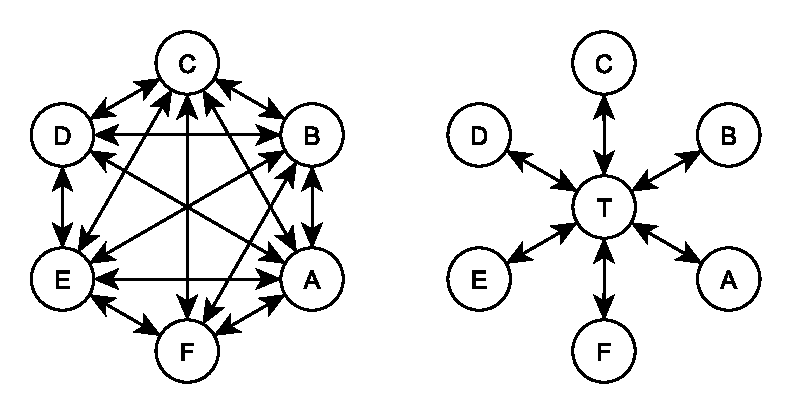
\includegraphics[width=0.8\textwidth]{pic/key_distribution-networks}
    \caption{Варианты сетей без выделенного доверенного центра и с выделенным доверенным центром T\label{fig:key_distribution-networks}}
\end{figure}

Если говорить о требованиях к данному классу протоколов с точки зрения свойств безопасности, то <<идеальный>> протокол распространения ключей должен реализовывать следующие цели:
\begin{itemize}
    \item[G1] аутентификация сторон протокола;
    \item[G3] защита от повтора;
    \item[G7] аутентификация ключа;
    \item[G8] подтверждение владения [новым] ключом;
    \item[G9] совершенная прямая секретность;
    \item[G10] формирование новых ключей.
    \item[G11] ограниченная защита от атак отказа в обслуживании.
\end{itemize}

Разумеется, <<идеальный>> протокол должен быть устойчивым ко всем известным атакам, в том числе рассмотренным в разделе~\ref{section-protocols-attacks}.

\input{symmetric}

\section{Трёхпроходные протоколы}\label{section-three-pass-protocols}
\selectlanguage{russian}

Если между Алисой и Бобом существует канал связи, недоступный для модификации злоумышленником (то есть когда применима модель только пассивного криптоаналитика), то даже без предварительного обмена секретными ключами или другой информацией можно воспользоваться идеями, использованными ранее в криптографии на открытых ключах. После описания RSA в 1978 году, в 1980 Ади Шамир предложил использовать криптосистемы, основанные на коммутативных операциях, для передачи информации без предварительного обмена секретными ключами. Если предположить, что передаваемой информацией является выработанный одной из сторон секретный сеансовый ключ, то в общем виде мы получаем следующий трёхпроходной протокол.

\begin{figure}[thb]
	\centering
	\begin{sequencediagram}
		\newinst{Alice}{Alice}
		\newinst[2.5]{Bob}{Bob}

		\mess{Alice}{$  E_A \left( K \right) $}{Bob}
		\mess{Bob}{$ E_B \left( E_A \left( K \right) \right) $}{Alice}
		\mess{Alice}{$ E_B \left( K \right) $}{Bob}
	\end{sequencediagram}
	\caption{Диаграмма последовательности взаимодействия участников в трёхпроходных протоколах\label{fig:key_distribution-three-pass}}
\end{figure}

Предварительно:

\begin{itemize}
	\item Алиса и Боб соединены незащищённым каналом связи, открытым для прослушивания (но не для модификации) злоумышленником.
	\item Каждая из сторон имеет пару из открытого и закрытого ключей $K_A$, $k_A$, $K_B$, $k_B$ соответственно.
	\item Сторонами выбрана и используется коммутативная функция шифрования:
	\[\begin{array}{lll}
		D_{A} \left( E_{A} \left( X \right) \right)	= X                                       & \forall X, \left\{ K_A, k_a \right\}; \\
		E_{A} \left( E_{B} \left( X \right) \right)	= E_B \left( E_A \left( X \right) \right) & \forall ~ K_A, K_B, X.
	\end{array}\]
\end{itemize}

Диаграмма последовательности взаимодействия участников протокола показана на рис.~\ref{fig:key_distribution-three-pass}. Протокол состоит из трёх проходов с передачей сообщений (отсюда название) и одного заключительного, на котором Боб вычисляет сеансовый ключ.

\begin{protocol}
    \item[(1)] Алиса выбирает новый сеансовый ключ $K$
    \item[{}] $Alice \to \left\{ E_A \left( K \right) \right\} \to Bob$
    \item[(2)] $Bob \to \left\{ E_B \left( E_A \left( K \right) \right) \right\} \to Alice$
    \item[(3)] Алиса, используя коммутативность функции шифрования, <<исключает>> из сообщения Боба шифрование на своём ключе $K_A$:
	\[ D_A \left( E_B \left( E_A \left( K \right) \right) \right) = D_A \left( E_A \left( E_B \left( K \right) \right) \right) = E_B \left( K \right). \]
    \item[{}] $Alice \to \left\{ E_B \left( K \right) \right\} \to Bob$
    \item[(4)] Боб расшифровывает $D_B \left( E_B \left( K \right) \right) = K$
\end{protocol}

В результате работы протокола стороны получают общий секретный ключ $K$.

Общим недостатком всех подобных протоколов является отсутствие аутентификации сторон. Конечно, в случае пассивного криптоаналитика это не требуется, но в реальной жизни всё-таки нужно рассматривать все возможные модели (в том числе активного криптоаналитика) и использовать такие протоколы, которые предполагают взаимную аутентификацию сторон.

Также, в отличие, например, от схемы Диффи~---~Хеллмана, рассмотренной в разделе~\ref{section-protocols-diffie-hellman}, новый ключ выбирается инициатором сеанса. Это позволяет инициатору, исходя не из лучших побуждений, заставить второго участника использовать устаревший сеансовый ключ.

Если говорить в терминах свойств безопасности, то все представители данного класса протоколов декларируют только аутентификацию ключа (G7). В отличие от схемы Диффи~---~Хеллмана, трёхпроходные протоколы не требуют выбора новых <<мастер>>-ключей для каждого сеанса протокола, из-за чего нельзя гарантировать ни совершенную прямую секретность (G9), ни формирование новых ключей (G10).

\subsection{Тривиальный вариант}

Приведём пример протокола на основе функции XOR (побитовое сложение по модулю 2). Хотя данная функция может использоваться как фундамент для построения систем совершенной криптостойкости (см. главу~\ref{chapter:perfect_secure_systems}), для трёхпроходного протокола это неудачный выбор. Продемонстрируем это далее.

Пусть перед началом протокола обе стороны имеют свои секретные ключи $K_A$ и $K_B$, представляющие собой случайные двоичные последовательности с равномерным распределением символов. Функция шифрования определяется как $E_i( X ) = X \oplus K_i$, где $X$ это сообщение, а $K_i$ -- секретный ключ. Очевидно, что:

\[ \begin{matrix}
\forall i, j, X: E_i \left( E_j \left( X \right) \right) & = & X \oplus K_j \oplus K_i & = & \\ 
 & = & X \oplus K_i \oplus K_j & = & E_j \left( E_i \left( X \right) \right).
\end{matrix}
\]

Протокол состоит из следующих проходов и действий.

\begin{figure}[thb]
	\centering
	\begin{sequencediagram}
		\newinst{Alice}{Alice}
		\newinst[2.5]{Bob}{Bob}
		
		\mess{Alice}{$  K \oplus K_A $}{Bob}
		\mess{Bob}{$ K \oplus K_A \oplus K_B $}{Alice}
		\mess{Alice}{$ K \oplus K_B $}{Bob}
	\end{sequencediagram}
	\caption{Диаграмма последовательности взаимодействия участников в тривиальном трёхпроходном протоколе}
\end{figure}

\begin{protocol}
    \item[(1)] Алиса выбирает новый сеансовый ключ $K$
    \item[{}] $Alice \to \left\{ E_A \left( K \right) = K \oplus K_A \right\} \to Bob$
    \item[(2)] $Bob \to \left\{ E_B \left( E_A \left( K \right) \right) = K \oplus K_A \oplus K_B \right\} \to Alice$
    \item[(3)] Алиса, используя коммутативность функции шифрования,
	\[ D_A \left( E_B \left( E_A \left( K \right) \right) \right) = K \oplus K_A \oplus K_B \oplus K_A = K \oplus K_B = E_B \left( K \right). \]
    \item[{}] $Alice \to \left\{ E_B \left( K \right) = K \oplus K_B \right\} \to Bob$
    \item[(4)] Боб расшифровывает $D_B \left( E_B \left( K \right) \right) = K \oplus K_B \oplus K_B = K$
\end{protocol}

По окончании сеанса протокола Алиса и Боб знают общий сеансовый ключ $K$.

Предложенный выбор коммутативной функции шифрования совершенной секретности является неудачным, так как существуют ситуации, при которых криптоаналитик может определить ключ $K$. Предположим, что криптоаналитик перехватил все три сообщения:
    \[ K \oplus K_A, ~~ K \oplus K_A \oplus K_B, ~~ K \oplus K_B. \]
Сложение по модулю 2 всех трёх сообщений даёт ключ $K$. Поэтому такая система шифрования не применяется.

Теперь приведём протокол надёжной передачи секретного ключа, основанный на экспоненциальной (коммутативной) функции шифрования. Стойкость этого протокола связана с трудностью задачи вычисления дискретного логарифма: при известных значениях $y, g, p$, найти $x$ из уравнения $y = g^x \bmod p$.

\subsection{Бесключевой протокол Шамира}\index{протокол!Шамира бесключевой|(}\label{section-protocols-shamir}

Стороны предварительно договариваются о большом простом числе $p \sim 2^{1024}$. Каждая из сторон выбирает себе по секретному ключу $a$ и $b$. Эти ключи меньше и взаимно просты с $p-1$. Также стороны приготовили по специальному числу $a'$ и $b'$, которые позволяют им расшифровать сообщение, зашифрованное своим ключом:
\[\begin{array}{l}
a' = a{-1} \mod (p-1), \\
a \times a' = 1 \mod (p-1), \\
\forall X: (X^a)^{a'} = X. \\
\end{array}\]

Последнее выражение верно по следствию из малой теоремы Ферма\index{теорема!Ферма малая}. Операции шифрования и расшифрования определяются следующим образом:
\[\begin{array}{lll}
\forall M < p: & C = E( M ) = M^{a}            & \mod p, \\
               & D( C ) = C^{a'}               & \mod p, \\
               & D_A( E_A( M ) ) = M^{aa'} = M & \mod p. \\
\end{array}\]

\begin{figure}[thb]
	\centering
	\begin{sequencediagram}
		\newinst{Alice}{Alice}
		\newinst[2.5]{Bob}{Bob}

		\mess{Alice}{$ K^a \bmod p $}{Bob}
		\mess{Bob}{$ K^{ab} \bmod p $}{Alice}
		\mess{Alice}{$ K^b \bmod p $}{Bob}
	\end{sequencediagram}
	\caption{Диаграмма последовательности взаимодействия участников в бесключевом протоколе Шамира}
\end{figure}

\begin{protocol}
    \item[(1)] Алиса выбирает новый сеансовый ключ $K < p$
    \item[{}] $Alice \to \left\{ E_A \left( K \right) = K^a \bmod p \right\} \to Bob$
    \item[(2)] $Bob \to \left\{ E_B \left( E_A \left( K \right) \right) = K^{ab} \bmod p \right\} \to Alice$
    \item[(3)] Алиса, используя коммутативность функции шифрования,
	\[ D_A \left( E_B \left( E_A \left( K \right) \right) \right) = K^{aba'} = K^b = E_B \left( K \right) \mod p. \]
    \item[{}] $Alice \to \left\{ E_B \left( K \right) = K^b \bmod p \right\} \to Bob$
    \item[(4)] Боб расшифровывает $D_B \left( E_B \left( K \right) \right) = K^{bb'} \bmod p = K$
\end{protocol}

По окончании сеанса протокола Алиса и Боб знают общий сеансовый ключ $K$.

Предположим, что криптоаналитик перехватил три сообщения:
\[ \begin{array}{l}
    y_1 = K^a \bmod p, \\
    y_2 = K^{ab} \bmod p, \\
    y_3 = K^b \bmod p. \\
\end{array} \]

Чтобы найти ключ $K$, криптоаналитику надо решить систему из этих трёх уравнений, что имеет очень большую вычислительную сложность, неприемлемую с практической точки зрения, если все три числа $a, b, ab$ достаточно велики. Предположим, что $a$ (или $b$) мало. Тогда, вычисляя последовательные степени $y_3$ (или $y_1$), можно найти $a$ (или $b$), сравнивая результат с $y_2$. Зная $a$, легко найти $a^{-1}\mod(p-1)$ и $K=(y_1)^{a^{-1}}\mod p$.

\index{протокол!Шамира бесключевой|)}

\subsection{Криптосистема Мэсси~---~Омуры}\index{протокол!Мэсси~---~Омуры|(}\index{криптосистема!Мэсси~---~Омуры|(}

В 1982 году Джеймс Мэсси и Джим Омура заявили патент (\langen{James Massey, Jim K. Omura},~\cite{Massey:Omura:1986}), улучшающий (по их мнению) бесключевой протокол Шамира. В качестве операции шифрования вместо возведения в степень в мультипликативной группе $\Z_p^*$ они предложили использовать возведение в степень в поле Галуа $\GF{2^n}$. Секретный ключ каждой стороны (для Алисы -- $a$) должен удовлетворять условиям:
\[ \begin{array}{l}
 a \in \GF{2^n}, \\
 gfd \left( a, x^{ n-1 } + x^{ n-2 } + ... + x + 1 \right) = 1. \\
\end{array} \]

В остальном протокол выглядит аналогично.

\index{протокол!Мэсси~---~Омуры|)}\index{криптосистема!Мэсси~---~Омуры|)}

\section{<<Криптосистемы-протоколы>>}\label{section-cryptosystems-protocols}
\selectlanguage{russian}

Как и создатели трёхпроходных протоколов из раздела~\ref{section-three-pass-protocols}, авторы следующих алгоритмов считали их не просто математическими конструкциями, обеспечивающие некоторую элементарную операцию (например, шифрование с открытым ключом), но пытались вокруг одной-двух математических конструкций построить законченную систему распространения ключей. Некоторые из этих конструкций, преобразовавшись, используются до настоящего времени (например, протокол Диффи-Хеллмана), некоторые -- остались только в истории криптографии и защиты информации.

Позже в 1990-х годах будут разделены математические асимметричные примитивы (шифрование и электронная подпись) и протоколы, эти примитивы использующие, что будет продемонстрировано в разделе~\ref{section-protocols-asymmetric}.

\subsection{Протокол Диффи~---~Хеллмана}\index{протокол!Диффи~---~Хеллмана}\label{section-protocols-diffie-hellman}
\selectlanguage{russian}

Первый алгоритм с открытым ключом был предложен Диффи и Хеллманом в работе 1976 года <<Новые направления в криптографии>> (\langen{Bailey Whitfield Diffie, Martin Edward Hellman, ``New directions in cryptography''},~\cite{Diffie:Hellman:1976}). Данный протокол, который также можно назвать \emph{схемой Диффи~---~Хеллмана}, стал первым, позволивший уменьшить требования к каналу связи для установления защищённого соединения без предварительного обмена ключами.

Протокол позволяет двум сторонам создать общий сеансовый ключ используя такой канал связи, который может прослушивать злоумышленник, но в предположении, что последний не может менять содержимое сообщений.

Пусть $p$ -- большое простое число\index{число!простое}, $g$ -- примитивный элемент группы $\Z_p^*$, ~ $y = g^x \bmod p$, причём $p, y, g$ известны заранее. Функцию $y=g^{x} \bmod p$ считаем однонаправленной, то есть вычисление функции при известном значении аргумента является лёгкой задачей, а её обращение (нахождение аргумента) при известном значении функции -- трудной.\footnote{Обратную функцию $x = \log_g y \bmod p$ называют функцией дискретного логарифма. В настоящий момент не существует быстрых способов вычисления такой функции для больших простых $p$.}

Протокол обмена состоит из следующих действий.

\begin{figure}
    \centering
    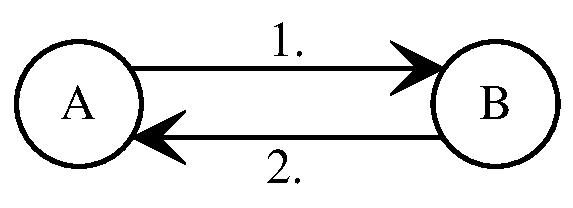
\includegraphics[width=0.5\textwidth]{pic/key_distribution-diffie-hellman}
    \caption{Общая схема взаимодействия участников в протоколе Диффи~---~Хеллмана\label{fig:key_distribution-diffie-hellman}}
\end{figure}

\begin{protocol}
    \item[(1)] Алиса выбирает случайное $2 \leq a \leq p - 1$
    \item[{}] $Alice \to \left\{ A = g ^ a \bmod p \right\} \to Bob$
    \item[(2)] Боб выбирает случайное $2 \leq b \leq p-1$
    \item[{}] Боб вычисляет сеансовый ключ $K = A ^ b \bmod p$
    \item[{}] $Bob \to \left\{ B = g ^ b \bmod p \right\} \to Alice$
    \item[(3)] Алиса вычисляет $K = B ^ a \bmod p$
\end{protocol}

Таким способом создан общий секретный сеансовый ключ $K$. За счёт случайного выбора значений $a$ и $b$ в новом сеансе будет получен новой сеансовый ключ.

Протокол обеспечивает только генерацию новых сеансовых ключей (цель G10). В отсутствие третей доверенной стороны он не обеспечивает ни аутентификацию сторон (цель G1), из-за отсутствия проходов с подтверждением владения ключом отсутствует аутентификация ключа (цель G8). Зато, так как протокол не использует длительные <<мастер>>-ключи, можно говорить о том, что он обладает свойством совершенной прямой секретности (цель G9).

Протокол можно использовать только с такими каналами связи, в которые не может вмешаться активный криптоаналитик. В противном случае протокол становится уязвим к простой <<атаке посередине>>.

\begin{figure}
    \centering
    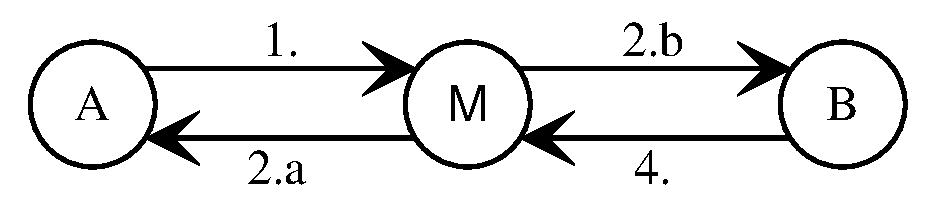
\includegraphics[width=0.67\textwidth]{pic/key_distribution-diffie-hellman-mitm}
    \caption{Схема взаимодействия участников в протоколе Диффи~---~Хеллмана в модели с активным криптоаналитиком\label{fig:key_distribution-diffie-hellman-mitm}}
\end{figure}

\begin{protocol}
    \item[(1)] Алиса выбирает случайное $2 \leq a \leq p - 1$
    \item[{}] $Alice \to \left\{ A = g ^ a \bmod p \right\} \to Mellory~(Bob)$
    \item[(2)] Меллори выбирает случайное $2 \leq m \leq p-1$
    \item[{}] Меллори вычисляет сеансовый ключ для канала с Алисой
        \[K_{AM} = A ^ m \bmod p = g ^ {am} \bmod p\]
    \item[{}] $Mellory~(Alice) \to \left\{ M = g ^ m \bmod p \right\} \to Bob$
    \item[{}] $Mellory~(Bob) \to \left\{ M = g ^ m \bmod p \right\} \to Alice$
    \item[(3)] Алиса вычисляет сеансовый ключ для канала с Меллори (думая, что Меллори это Боб)
        \[K_{AM} = M ^ a \bmod p = g ^ { am } \bmod p\]
    \item[(4)] Боб выбирает случайное $2 \leq b \leq p-1$
    \item[{}] Боб вычисляет сеансовый ключ для канала с Меллори (думая, что Меллори это Алиса)
        \[K_{BM} = M ^ b \bmod p = g ^ { bm } \bmod p\]
    \item[{}] $Bob \to \left\{ B = g ^ b \bmod p \right\} \to Mellory~(Alice)$
    \item[(5)] Меллори вычисляет сеансовый ключ для канала с Бобом
        \[K_{BM} = B ^ m \bmod p = g ^ { bm } \bmod p\]
\end{protocol}

В результате Алиса и Боб получили новые сеансовые ключи, но <<защищённый>> канал связи установили не с друг с другом, а со злоумышленником, который теперь имеет возможность ретранслировать или изменять все передаваемые сообщения между Алисой и Бобом.

Протокол Диффи~---~Хеллмана отличается от большей части протоколов распространения ключей из-за того, что не использует другие криптографические примитивы (функции шифрования, электронно-цифровой подписи или хеширования), но сам по себе является в некотором смысле криптографическим примитивом для построения более сложных протоколов. Он обеспечивает генерацию случайного числа в распределённой системе без доверенного центра. Причём ни одна из сторон не может заставить другую сторону использовать старый сессионный ключ, в отличие от, например, протокола Yahalom\index{протокол!Yahalom} из раздела~\ref{section-protocols-yahalom}.

Протокол можно изменить таким образом, чтобы вместо мультипликативной группы простого умножения использовать аддитивную группу сложения точек эллиптической кривой (см. раздел~\ref{section-math-ec-groups}). В этом случае стороны по прежнему будут выбирать некоторые случайные целые числа, но не возводить генератор-число в степень, а умножать генератор-точку на загаданное число.

\begin{protocol}
    \item[(0)] Стороны договорились о группе точек эллиптической кривой $\group{E}$, её циклической подгруппе $\group{G}$ мощности $n = \| \group{G} \|$ и генераторе $G$ группы $\group{G}$ (или хотя бы достаточно большой подгруппы группы $\group{G}$).
    \item[(1)] Алиса выбирает случайное $2 \leq a \leq n - 1$
    \item[{}] $Alice \to \left\{ A = a \times G \right\} \to Bob$
    \item[(2)] Боб выбирает случайное $2 \leq b \leq n - 1$
    \item[{}] Боб вычисляет точку $K = b \times A$
    \item[{}] $Bob \to \left\{ B = g \times G \right\} \to Alice$
    \item[(3)] Алиса вычисляет точку $K = a \times B$
\end{protocol}

В качестве нового сессионного ключа стороны могут выбрать, например, первую координату найденной точки $K$.


\section{Системы Эль-Гамаля}
\selectlanguage{russian}

\subsection[Шифрование]{Система шифрования Эль-Гамаля}

Эта система шифрования с открытым ключом опубликована Эль-Гамалем (El-Gamal) в 1985 году. Рассмотрим принципы ее построения.

Пусть имеется мультипликативная группа $\Z_p^* = \{1, 2, \dots, p-1\}$, где $p$ -- большое простое число, содержащее 1024 двоичных разряда. Существует целое число $g$, называемое примитивным элементом, который порождает все ненулевые числа группы, причем $1 < g < p-1$.

    \[ g\mod p, ~~ g^2\mod p, ~~ \dots, ~~ g^{p-1} = 1\mod p \]

Выберем целое число $x$ в интервале $1 \le x \le p-1$. Вычислим
    \[ y = g^x \mod p. \]
Известно, что в конечном поле функция $y(x)$ -- вычислительно однонаправленная.

Задачей \textbf{дискретного логарифмирования}\index{задача!дискретного логарифмирования} в мультипликативной группе $\Gr$ называется нахождение $x$ по заданным элементам $a,b \in \Gr, ~ b = a^x$. Для групп большого размера $2^{150}$--$2^{1000}$ при выборе элемента $a$ генератором группы или подгруппы большого порядка дискретный логарифм известными алгоритмами не вычислим за доступное время, все известные алгоритмы -- неполиномиальные.

Процедура шифрования криптосистемы  Эль-Гамаля состоит из следующих операций.

\begin{enumerate}
    \item \textbf{Создание пары из секретного и открытого ключей стороной $A$.}
        \begin{enumerate}
            \item $A$ выбирает простое случайное число $p$.
            \item Выбирает генератор $g$ (в программных реализациях алгоритма генератор часто выбирается малым числом, например $g = 2 \mod p$).
            \item Выбирает $x \in [1, p-1]$ с помощью генератора случайных чисел.
            \item Вычисляет $y=g^{x}\mod p$,
            \item Создает секретный и открытые ключи $\SK$ и $\PK$:
                \[ \SK = (x), ~ \PK = (p, g, y). \]
                Криптостойкость задается битовой длиной параметра $p$.
        \end{enumerate}
    \item \textbf{Шифрование на открытом ключе стороной $B$.}
        \begin{enumerate}
            \item $B$ извлекает открытый ключ $\text{PK} = (p, g, y)$ из директории стороны $A$.
            \item Сообщение представляется числом $m \in [1,p-1]$.
            \item Выбирает случайное число $r \in [1, p-1]$ и вычисляет
                \[ \begin{array}{l}
                    a = g^r \mod p, \\
                    b = m y^r \mod p.
                \end{array} \]
            \item Создает шифрованное сообщение в виде
                \[ c = (a,b) \]
                и посылает стороне $A$.
        \end{enumerate}
    \item \textbf{Расшифрование на секретном ключе стороной $A$.}
        \begin{enumerate}
            \item Используя секретный ключ $x$, $A$ вычисляет
                \[ m = \frac{b}{a^x} \mod p. \]
            \item Расшифрование корректно, так как
                \[ \begin{array}{l}
                    \frac{b}{a^x} = \frac{m y^r}{g^{rx}} = m \mod p, \\
                    m \mod p \equiv m.
                \end{array} \]
        \end{enumerate}
\end{enumerate}


\subsubsection{Пример системы}

\begin{enumerate}
    \item Генерирование параметров.
        \begin{enumerate}
            \item Выберем $p=41$.
            \item Группа $\Z_p^*$ циклическая, найдем генератор (примитивный элемент). Порядок группы
                \[ |\Z_p^*| = \phi(p) = p-1 = 40. \]
                Делители 40: 2, 4, 5, 8, 10, 20. Элемент группы является примитивным, если все его степени, соответствующие делителям порядка группы, не сравнимы с 1. Из табл. \ref{tab:elgamal-generator-search} видно, что число $g = 6$ является генератором всей группы.
                \begin{table}[h!]
                    \centering
                    \caption{Поиск генератора в циклической группе $\Z_{41}^*$. Элемент 6 -- генератор\label{tab:elgamal-generator-search}}
                    \resizebox{\textwidth}{!}{ \begin{tabular}{|c|c|c|c|c|c|c|c|c|}
                        \hline
                        \multirow{2}{*}{Элемент} & \multicolumn{7}{|c|}{Степени} & \multirow{2}{*}{Порядок элемента} \\
                        \cline{2-8}
                                & 2   & 4   & 5   & 8  & 10 & 20 & 40 & \\
                        \hline
                        2       & 4   & 16  & -9  & 10 & -1 & 1  &    & 20 \\
                        3       & 9   & -1  & -3  & 1  &    &    &    & 8 \\
                        5       & -16 & 10  & 9   & 18 & -1 & 1  &    & 20 \\
                        6       & -5  & -16 & -14 & 10 & -9 & -1 & 1  & 40 \\
                        \hline
                    \end{tabular} }
                \end{table}
            \item Выберем случайное $x = 19 \in [1, p-1]$.
            \item Вычислим
                \[ \begin{array}{ll}
                    y & = g^x \mod p = \\
                    & = 6^{19} \mod 41 = \\
                    & = 6^{1 + 2 + 4 \cdot 0 + 8 \cdot 0 + 16} \mod 41 = \\
                    & = 6^1 \cdot 6^2 \cdot 6^{4 \cdot 0} \cdot 6^{8 \cdot 0} \cdot 6^{16} \mod 41 = \\
                    & = 6 \cdot (-5) \cdot (-16)^0 \cdot 10^0 \cdot 18 \mod 41 = \\
                    & = -7 \mod 41.
                \end{array} \]
            \item Открытый и секретные ключи:
                \[ \PK = (p:41, g:6, y:-7), ~ \SK = (x:19). \]
        \end{enumerate}
    \item Шифрование.
        \begin{enumerate}
            \item Пусть сообщением является число $m = 3 \in \Z_p^*$.
            \item Выберем случайное число $r = 25 \in [1, p-1]$.
            \item Вычислим
                \[ \begin{array}{l}
                    a = g^r \mod p = 6^{25} \mod 41 = 14 \mod 41, \\
                    b = m y^r \mod p = 3 \cdot (-7)^{25} \mod 41 = -9 \mod 41.
                \end{array} \]
            \item Шифротекстом является пара чисел
                \[ c = (a:14, ~ b:-9). \]
        \end{enumerate}
    \item Расшифрование.
        \begin{enumerate}
            \item Пусть получен шифротекст
                \[ c = (a:14, ~ b:-9). \]
            \item Вычислим открытый текст как
                \[ \begin{array}{ll}
                    m & = \frac{b}{a^x} \mod p = \\
                    & = -9 \cdot (14^{-1})^{19} \mod 41 = \\
                    & = -9 \cdot 3^{19} \mod 41 = \\
                    & = -9 \cdot (-14) \mod 41 = \\
                    & = 3 \mod 41. \\
                \end{array} \]
        \end{enumerate}
\end{enumerate}


\subsection[Электронная цифровая подпись]{Электронная цифровая подпись \protect\\ Эль-Гамаля}

Криптосистема Эль-Гамаля, как и криптосистема RSA,  может быть использована для создания ЭЦП.

По-прежнему имеются два пользователя $A$ и $B$ и незащищенный канал связи между ними. Пользователь $A$  хочет подписать свое открытое сообщение $m$  для того, чтобы пользователь $B$ мог убедиться, что именно $A$ подписал сообщение.

Пусть $A$ имеет секретный ключ $\SK = (x)$, открытый ключ $\PK = (p,g,y)$ (полученные так же, как и в системе шифрования Эль-Гамаля) и хочет подписать открытое сообщение. Обозначим подпись $S(m)$.

Для создания подписи $S(m)$ пользователь $A$ выполняет следующие операции:
\begin{itemize}
    \item вычисляет значение криптографической хэш-функции  $h(m) \in [0,p-2]$, от своего открытого сообщения $m$;
    \item выбирает случайное число $r, ~ \gcd(r, p-1)=1$;
    \item используя открытый ключ, вычисляет
        \[ \begin{array}{l}
            a = g^r \mod p, \\
            b = \frac{h(m) - xa}{r} \mod (p-1); \\
        \end{array} \]
    \item создает подпись в виде двух чисел
        \[ S(m) = (a, b) \]
        и посылает сообщение с подписью $(m, S(m))$.
\end{itemize}

Получив сообщение,  $B$ осуществляет проверку подписи, выполняя следующие операции:
\begin{itemize}
    \item по известному сообщению $m$ вычисляет значение хэш-функции $h(m)$;
    \item вычисляет
        \[ \begin{array}{l}
            f_1 = g^{h(m)} \mod p, \\
            f_2 = y^a a^b \mod p; \\
        \end{array} \]
    \item сравнивает значения $f_1$ и $f_2$, если
        \[ f_1 = f_2, \]
        то подпись подлинная, в противном случае -- фальсифицированная (или случайно испорченная).
\end{itemize}

Покажем, что проверка подписи корректна. По малой теореме Ферма получаем
\[ \begin{array}{ll}
    f_1 & = g^{h(m)} \mod p = \\
    & \\
    & = g^{h(m) \mod (p-1)} \mod p; \\
\end{array} \] \[ \begin{array}{ll}
    f_2 & = y^a a^b \mod p = \\
    & = \underbrace{\left( g^x \right)^a}_{y^a} \cdot
        \underbrace{\left( g^r \mod p \right)^{\frac{h(m) - xa}{r} \mod (p-1)}}_{a^b} \mod p = \\
    & \\
    & = g^{xa \mod (p-1)} ~\cdot~ g^{h(m) - xa \mod (p-1)} \mod p = \\
    & = g^{h(m) \mod (p-1)} \mod p = \\
    & = f_1.
\end{array} \]

\subsubsection{Пример системы}

\begin{enumerate}
    \item Генерирование параметров.
        \begin{enumerate}
            \item Выберем $p=41$.
            \item Выберем генератор $g=6$ в группе $\Z_{41}^*$.
            \item Выберем случайное $x = 19 \in [1, p-1]$.%, ~ \gcd(x, p-1) = 1$.
            \item Вычислим
                \[ \begin{array}{ll}
                    y & = g^x \mod p = \\
                    & = 6^{19} \mod 41 = \\
                    & = 6^{1 + 2 + 4 \cdot 0 + 8 \cdot 0 + 16} \mod 41 = \\
                    & = 6 \cdot (-5) \cdot (-16)^0 \cdot 10^0 \cdot 18 \mod 41 = \\
                    & = -7 \mod 41. \\
                \end{array} \]
            \item Открытый и секретные ключи:
                \[ \PK = (p:41, g:6, y:-7), ~ \SK = (x:19). \]
        \end{enumerate}
    \item Подписание.
        \begin{enumerate}
            \item От сообщения $m$ вычисляется хэш $h = H(m)$. Пусть хэш $h  = 3 \in [0, p-2]$.
            \item Выберем случайное $r = 9 \in [1, p-2]$: \\
                $\gcd(r=9, p-1 = 40) = 1$.
            \item Вычислим
                \[ \begin{array}{ll}
                    a & = g^r \mod p = \\
                      & = 6^9 \mod 41 = 19 \mod 41, \\
                    b & = \frac{h - xa}{r} \mod (p-1) = \\
                      & = (3 - 19 \cdot 19) \cdot 9^{-1} \mod 40 = \\
                      & = 2 \cdot 9 \mod 40 = 18 \mod 40. \\
                \end{array} \]
            \item Подпись
                \[ s = (a:19, b:18). \]
        \end{enumerate}
    \item Проверка подписи.
        \begin{enumerate}
            \item Для полученного сообщения находится хэш $h = H(m) = 3$. Пусть полученная подпись к нему имеет вид
                \[ s = (a:19, b:18). \]
            \item Вычислим
                \[ \begin{array}{ll}
                    f_1 & = g^h \mod p = \\
                        & = 6^3 \mod 41 = 11 \mod 41, \\
                    f_2 & = y^a a^b \mod p = \\
                        & = (-7)^{19} \cdot 19^{18} \mod 41 = 11 \mod 41. \\
                \end{array} \]
            \item Проверим равенство $f_1$ и $f_2$. Подпись верна, так как
                \[ f_1 = f_2 = 11. \]
        \end{enumerate}
\end{enumerate}


\subsection[Криптостойкость]{Криптостойкость систем \protect\\ Эль-Гамаля}

Пусть дано уравнение $y=g^{x} \mod p$, требуется определить $x$ в интервале $0<x<p-1$. Задача называется \textbf{дискретным логарифмированием}\index{задача!дискретного логарифма}.

Рассмотрим возможные способы нахождения неизвестного числа $x$. Начнем с перебора различных значений $x$ из интервала $0<x<p-1$ и проверке равенства $y=g^{x} \mod p$. Число попыток в среднем равно $\frac{p}{2}$, при $p=2^{1024}$ это число равно $2^{1023}$, что на практике не осуществимо.

Другой подход предложен советским математиком Гельфондом\index{алгоритм!Гельфонда} безотносительно к криптографии. Он состоит в следующем.
Вычислим $S=\lceil\sqrt{p-1}\rceil $, где скобки означают ближайшее (сверху) целое от числа $\sqrt{p-1} $.

Представим искомое число $x$   в следующем виде

\begin{equation}
    x=x_{1} S+x_{2},
    \label{S}
\end{equation}

где $x_{1}$ и $x_{2}$ -- целые неотрицательные числа,
    \[ x_{1} \le S-1, ~ x_{2} \le S-1. \]
Такое представление является однозначным.

Вычислим и занесем в таблицу следующие $S$  чисел:
    \[ g^{0} \mod p, ~~ g^{1} \mod p, ~~ g^{2} \mod p, ~~ \dots, ~~ g^{S-1} \mod p. \]
Вычислим $g^{-S} \mod p$ и также занесем в таблицу.

\begin{center} \begin{tabular}{|l|c|c|c|c|c|c|}
    \hline
    $\lambda $ & 0 & 1 & 2 & \dots & $S-1$ & $-S$ \\
    \hline
    $g^{\lambda} \mod p$ & $g^{0}$ & $g^{1}$ & $g^{2}$ & \dots & $g^{S-1}$ & $g^{-S}$ \\
    \hline
\end{tabular} \end{center}

Для решения уравнения \ref{S} используем перебор значений $x_{1}$.
\begin{enumerate}
    \item  Предположим, что $x_{1} = 0$. Тогда $x = x_{2}$.  Если число $y = g^{x_{2}} \mod p$ содержится в таблице, то  находим его и выдаем результат: $x=x_{2} $. Задача решена. В противном случае переходим к пункту 2.
    \item  Предположим, что $x_{1} =1$. Тогда $x=S+x_{2} $ и $y=g^{S+x_{2}} \mod p$. Вычисляем $yg^{-S} \mod p=g^{x_{2}} \mod p$. Задача сведена к предыдущей: если $g^{x_{2} } \mod p$ содержится в таблице, то в таблице находим число $x_{2} $ и выдаем результат $x$: $x=S+x_{2} $.
    \item  Предположим, что $x_{1} =2$. Тогда $x=2S+x_{2} $ и $y=g^{2S+x_{2} } \mod p$. Если число $yg^{-2S} \mod p=g^{x_{2} } \mod p$ содержится в таблице, то находим число $x_{2}$ и выдаем результат: $x = 2S + x_{2}$.
     \item  Пробегая все возможные значения, доберемся, в худшем случае, до $x_{1} =S-1$. Тогда $x=(S-1)S+x_{2} $ и $y = g^{(S-1)S+x_{2} } \mod p$. Если число $yg^{-(S-1)S} \mod p=g^{x_{2}} \mod p$ содержится в таблице, то  находим его и выдаем результат: $x=(S-1)S+x_{2}$.
\end{enumerate}

Легко проверить, что с помощью построенной таблицы мы проверили все возможные значения $x$. Максимальное число умножений равно $2S \approx 2\sqrt{p-1} =2\times 2^{512} $, что для практики очень велико.  Тем самым проблему достаточной криптостойкости этой системы можно было бы считать решенной. Однако это не верно, так как числа $p-1$ являются составными. Если  $p-1$ можно разложить на маленькие множители, то криптоаналитик может применить процедуру, подобную процедуре Гельфонда, по взаимно простым делителям  $p-1$  и найти секрет. Пусть  $p-1=st$. Тогда элемент $g^s$ образует подгруппу порядка $t$ и наоборот. Теперь, решая уравнение $y^s=(g^s)^a\mod p$, находим вычет $x=a\mod t$. Поступая аналогично, находим $x=b\mod s$ и по Китайской теореме об остатках находим $x$.

Несколько позже подобный метод ускоренного решения уравнения \ref{S} был предложен Шенксом (Shanks)и Хеллманом (Hellman). В англоязычной технической литературе он получил название алгоритма Шенкcа.

Пусть $k = \lceil \log_2 p \rceil$ -- битовая длина числа $p$. Алгоритм Гельфонда имеет  экспоненциальную сложность (число двоичных операций)
    \[ O(\sqrt{p}) = O(e^{\frac{1}{2} \frac{1}{\log_2 e} k}). \]

Наилучшие из известных алгоритмов решения задачи дискретного логарифма имеют экспоненциальную сложность порядка
    \[ O(e^{\sqrt{k}}). \]


\subsection{Взаимная аутентификация шифрованием}
\selectlanguage{russian}

К протоколам взаимной аутентификации принадлежит семейство протоколов, разработанных Т. Мацумото (T. Matsumoto), И. Такашима (Y. Takashima) и Х. Имаи (H. Imai) и названных по первым буквам фамилий авторов -- \textbf{протокол MTI}\index{протокол!MTI}.

Здесь к открытым данным относятся
    \[ p, ~~ g, ~~ \PK_A = g^a \mod p, ~~ \PK_B = g^b \mod p. \]
Каждый пользователь $A$ и $B$ обладает парой долговременных ключей для \emph{схемы шифрования с открытым ключом}: закрытый ключ расшифрования $\SK$ и открытый ключ шифрования  $\PK$.
\[ \begin{array}{ll}
    A: & ~ \SK_A = a, ~~ \PK_A = g^a \mod p, \\
    B: & ~ \SK_B = b, ~~ \PK_B = g^b \mod p. \\
\end{array} \]

\textbf{Протокол MTI}:
\begin{enumerate}
    \item Сторона $A$ генерирует случайное число $x, ~ 2\leq x\leq p-1$, создает и отправляет $B$ сообщение:
        \[ A \rightarrow B: ~ g^x \mod p. \]
    \item Сторона $B$ генерирует случайное число $y, ~ 2\leq y\leq p-1$, создает и отправляет $A$ сообщение:
        \[ A \leftarrow B: ~ g^y \mod p. \]
    \item Сторона $A$, используя открытые данные и полученное сообщение, создает сеансовый ключ:
        \[ K_A = (g^b)^x \cdot (g^y)^a = g^{bx+ay} \mod p. \]
    \item Сторона $B$, используя открытые данные и полученное сообщение, создает сеансовый ключ:
        \[ K_B = (g^x)^b \cdot (g^a)^y = g^{bx+ay} \mod p. \]
        Сеансовые ключи обоих сторон совпадают:
        \[ K_{A} =K_{B} = K. \]
\end{enumerate}

В описанном протоколе происходит взаимная аутентификация сторон как и в протоколе Эль-Гамаля\index{криптосистема!Эль-Гамаля}: открытые ключи сторон незаметно подменить невозможно. Наблюдая сообщения протокола, вычислить $g^{bx+ay}$ можно, только если известны значения $a,x$ или $b,y$, что представляет собой задачу дискретного логарифма, трудную в вычислительном смысле в настоящее время.


\subsection{Протокол Station-to-Station}\label{section-protocols-sts}\index{протокол!Station-to-Station|(}
\selectlanguage{russian}

Протокол STS (\langen{Station-to-Station},~\cite{Diffie:Oorschot:Wiener:1992})\index{протокол!Station-to-Station} предназначен для систем мобильной связи. Он использует идеи протокола Диффи~---~Хеллмана\index{протокол!Диффи~---~Хеллмана} и криптосистемы RSA\index{криптосистема!RSA}. Особенностью протокола является использование механизма электронной подписи\index{электронная подпись} для взаимной аутентификации сторон\index{аутентификация!взаимная}.

Предварительно стороны договорились об общих параметрах системы $p$ и $g$, где $p$ -- большое простое число, а $g$ -- примитивный элемент поля $\Z_p^*$.

Каждая из сторон $A$ и $B$ обладает долговременной парой ключей: закрытым ключом для расшифрования и создания электронной подписи $K_{\text{private}}$ и открытым ключом для шифрования и проверки подписи $K_{\text{public}}$.

\[\begin{array}{ll}
    A: K_{A,\text{private}}, K_{A,\text{public}}: \forall M : & \text{Verify}_A ( M, S_A( M ) ) = true, \\
                                                & D_A ( E_A( M ) ) = M, \\
    B: K_{B,\text{private}}, K_{B,\text{public}}: \forall M : & \text{Verify}_B ( M, S_B( M ) ) = true, \\
                                                & D_B ( E_B( M ) ) = M. \\
\end{array}\]

Где $\text{Verify}_A(\dots)$ это функция проверки электронной подписи на открытом ключе $K_{A, \text{public}}$, а $D_A$ -- функция расшифрования с использованием закрытого ключа $K_{A, \text{private}}$.

Протокол состоит из четырёх проходов, три из которых включают передачу сообщений (рис.~\ref{fig:key_distribution-sts}, \cite{Cheremushkin:2009}).

\begin{figure}
    \centering
    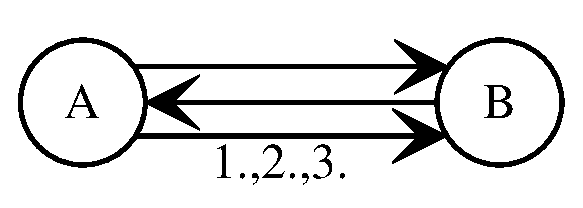
\includegraphics[width=0.5\textwidth]{pic/key_distribution-sts}
    \caption{Взаимодействие участников в протоколе STS\label{fig:key_distribution-sts}}
\end{figure}

\begin{protocol}
    \item[(1)] Алиса выбирает случайное число $R_A: 2 \leq R_A \leq p-1$.
    \item[{}] $Alice \to \left\{ A, m_A = g^{R_A} \bmod p \right\} \to Bob$

    \item[(2)] Боб выбирает случайное число $R_B: 2 \leq R_B \leq p-1$.
    \item[{}] Боб вычисляет сессионный ключ $K = m_A^{R_B} \bmod p$.
    \item[{}] $Bob \to \left\{ B, A, m_B = g^{R_B} \bmod p, E_K( S_B ( m_A, m_B )) \right\} \to Alice$

    \item[(3)] Алиса вычисляет сессионный ключ $K = m_B^{R_A} \bmod p$.
    \item[{}] Алиса проверяет подпись в сообщении $E_K( S_B ( m_A, m_B ))$.
    \item[{}] $Alice \to \left\{ A, B, E_K( S_A ( m_A, m_B ) ) \right\} \to Bob$

    \item[(4)] Боб проверяет подпись в сообщении $E_K( S_A ( m_A, m_B ))$.
\end{protocol}

Протокол обеспечивает гарантию формирования новых ключей (G10), но не совершенную прямую секретность (G9).

Как показала атака Лоу 1996 года (\cite{Lowe:1996}, рис.~\ref{fig:key_distribution-sts-attack}), протокол не может гарантировать аутентификацию субъектов (цель G1), ключей (G7) и подтверждение владения сессионным ключом (G8). Хотя злоумышленник не может получить доступ к новому сессионному ключу, если протокол использовать только для аутентификации субъектов, Алиса может принять злоумышленника за Боба.

\begin{figure}
    \centering
    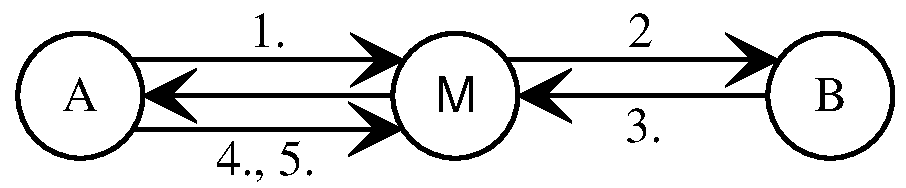
\includegraphics[width=0.67\textwidth]{pic/key_distribution-sts-attack}
    \caption{Схема взаимодействия участников в протоколе STS при атаке Лоу\label{fig:key_distribution-sts-attack}}
\end{figure}

\begin{protocol}
    \item[(1)] Алиса выбирает случайное число $R_A: 2 \leq R_A \leq p-1$.
    \item[{}] $Alice \to \left\{ A, m_A = g^{R_A} \bmod p \right\} \to Mellory~(Bob)$

    \item[(2)] $Mellory~(Alice) \to \left\{ M, m_A \right\} \to Bob$

    \item[(3)] Боб выбирает случайное число $R_B: 2 \leq R_B \leq p-1$ и вычисляет $m_B = g^{R_B} \bmod p$, а также сессионный ключ $K = m_A^{R_B} \bmod p$.
    \item[{}] $Bob \to \left\{ B, M, m_B, E_K( S_B ( m_A, m_B )) \right\} \to Mellory$

    \item[(4)] $Mellory~(Bob) \to \left\{ B, A, m_B, E_K( S_B ( m_A, m_B )) \right\} \to Alice$

    \item[(5)] Алиса вычисляет сессионный ключ $K = m_B^{R_A} \bmod p$.
    \item[{}] Алиса проверяет подпись в сообщении $E_K( S_B ( m_A, m_B ))$.
    \item[{}] $Alice \to \left\{ A, B, E_K( S_A ( m_A, m_B ) ) \right\} \to Mellory~(Bob)$
\end{protocol}

После успешного завершения протокола Алиса уверена, что общается с Бобом.

Как и все остальные <<криптосистемы-протоколы>>, протокол Station-to-Station основывается на некотором внешнем источнике информации об открытых ключах участников, не подвергая сомнению корректность и надёжность этого источника. Что, в общем случае, неверно. Если информацию о ключах участников нужно получать извне при каждом сеансе протокола (например, если участников много, и запомнить ключи всех возможности нет), то канал получения открытых ключей будет основной целью активного криптоаналитика для рассмотренных протоколов. Как от этого защититься с использованием примитивов асимметричной криптографии -- в разделе~\ref{section-protocols-asymmetric}.

\index{протокол!Station-to-Station|)}


\section{Схемы с доверенным центром}\label{key-distribution-schemas}\index{схема!распределения ключей|(}
\selectlanguage{russian}

Схемы распределения ключей с доверенным центром состоят из трёх этапов.

\begin{enumerate}
    \item На первом этапе доверенный центр создаёт некоторый секрет, известный только ему. Это может быть некоторая секретная матрица с особыми свойствами, как в схеме Блома\index{схема!Блома} из раздела~\ref{section-bloms-scheme}, или пара из закрытого и открытого ключей, как в схеме Жиро\index{схема!Жиро} из раздела~\ref{section-girault-scheme}.
    \item Для каждого нового легального участника сети доверенный центр, используя свою секретную информацию, вырабатывает некоторый отпечаток или сертификат, который позволяет новому участнику вырабатывать сеансовые ключи с другими легальными участниками.
    \item Наконец, на третьем этапе, когда начинается протокол общения двух легальных участников, они предъявляют друг-другу идентификаторы и/или дополнительную информацию от доверенного центра. Используя её, без дополнительного обращения к центру, они могут сгенерировать секретный сеансовый ключ для общения между собой.
\end{enumerate}

\subsection{Схема Жиро}\label{section-girault-scheme}\index{схема!Жиро|(}
\selectlanguage{russian}

В схеме Жиро (\langfr{Marc Girault},~\cite{Girault:1990, Girault:1991}) надёжность строится на стойкости криптосистемы RSA (сложности факторизации больших чисел и вычисления дискретного корня).

Предварительно:
\begin{itemize}
    \item Доверенный центр (Трент, $T$):
    \begin{itemize}
        \item выбирает общий модуль $n = p \times q$, где $p$ и $q$ -- большие простые числа;
        \item выбирает пару из закрытого и открытого ключей $K_{T, \text{public}}: (e, n)$ и $K_{T, \text{private}}: (d, n)$;
        \item выбирает элемент $g$ поля $\mathbb{Z}_n^{\times}$ максимального порядка;
        \item публикует в общедоступном месте параметры схемы $n$, $e$ и $g$.
    \end{itemize}
    \item Каждый из легальных участников:
    \begin{itemize}
        \item выбирает себе закрытый ключ $s_i$ и идентификатор $I_i$;
        \item вычисляет и отправляет доверенному центру $v_i = g^{-s_i} \bmod n$;
        \item используя протокол аутентификации сторон (см. ниже) легальный участник доказывает доверенному центру, что владеет закрытым ключом, не раскрывая его значение;
        \item получает от доверенного центр свой открытый ключ:
            \[ P_i = (v_i - I_i)^d = (g^{-s_i} - I_i)^d \mod n; \]
    \end{itemize}
    В результате для каждого участника, например, Алисы, которая владеет $P_A, I_A, s_a$ будет выполняться утверждение:
        \[ P_A^e + I_A = g^{-s_A} \mod n. \]
\end{itemize}

Протокол аутентификации сторон в общем случае выглядит следующим образом (рис.~\ref{fig:key_distribution-girault-auth}).

\begin{figure}
    \centering
    \includegraphics[width=0.5\textwidth]{pic/key_distribution-girault-auth}
    \caption{Взаимодействия участников в протоколе идентификации Жиро\label{fig:key_distribution-girault-auth}}
\end{figure}

\begin{protocol}
    \item[(1)] Алиса выбирает случайное $R_A$.
    \item[{}] $Alice \to \left\{ I_A, P_A, t = g^{R_A} \right\} \to Bob$
    \item[(2)] Боб выбирает случайное $R_B$.
    \item[{}] $Bob \to \left\{ R_B \right\} \to Alice$
    \item[(3)] $Alice \to \left\{ y = R_A + s_A \times R_B \right\} \to Bob$
    \item[(4)] Боб вычисляет $v_A = P_A^e + I_A$;
    \item[{}] Боб проверяет, что $g^ y v_A^{R_B} = t$.
\end{protocol}

Протокол генерации сессионного ключа, либо просто \emph{схема Жиро}, как и другие схемы, состоит из проходов обмена открытой информацией и вычисления ключа (рис.~\ref{fig:key_distribution-girault-scheme}).

\begin{figure}
    \centering
    \includegraphics[width=0.5\textwidth]{pic/key_distribution-girault-scheme}
    \caption{Взаимодействие участников в схеме Жиро\label{fig:key_distribution-girault-scheme}}
\end{figure}

\begin{protocol}
    \item[(1)] $Alice \to \left\{ P_A, I_A \right\} \to Bob$
    \item[(2)] Боб вычисляет $K_{BA} = (P_A^e + I_A)^{s_B} \bmod n$.
    \item[{}] $Bob \to \left\{ P_B, I_B \right\} \to Alice$
    \item[(3)] Алиса вычисляет $K_{AB} = (P_B^e + I_B)^{s_A} \bmod n$.
\end{protocol}

В результате работы схемы стороны сгенерировали одинаковый общий сеансовый ключ.
\[ K_{AB} = (P_A^e + I_A)^{s_B} = (g^{-s_A})^{s_B} = g^{-s_As_B} \mod n; \]
\[ K_{BA} = (P_B^e + I_B)^{s_A} = (g^{-s_B})^{s_A} = g^{-s_As_B} \mod n; \]
            \[ K = K_{AB} = K_{BA} = g^{-s_As_B} \mod n. \]

Схема обеспечивает аутентификацию ключа (цель G7), так как только легальные пользователи смогут вычислить корректное значение общего сессионного ключа.

\index{схема!Жиро|)}

\subsection{Схема Блома}\index{схема!Блома}
\selectlanguage{russian}

Рассмотрим распределение ключей по \emph{схеме Блома} (Rolf Blom,~\cite{Blom:1984, Blom:1985}), в котором каждые два пользователя из общего числа $N$ пользователей могут создать общий секретный ключ, причём секретные ключи каждой пары различны. Данная схема используется в протоколе HDCP\index{протокол!HDCP} (\langen{High-bandwidth Digital Content Protection}) для предотвращения копирования высококачественного видеосигнала.

На этапе инициализации доверенный центр выбирает симметричную матрицу $D_{m,m}$ над конечным полем $\GF p$. Для присоединения к сети распространения ключей новый участник либо самостоятельно, либо с помощью доверенного центра выбирает новый открытый ключ (идентификатор) $I$, представляющий собой вектор длины $k$ над $\GF p$. Доверенный центр вычисляет для нового участника закрытый ключ $K$:

\begin{equation}
	K = D_{m,m} I.
	\label{eq:blom_center_matrix}
\end{equation}

Симметричность матрицы $D_{m,m}$ доверенного центра позволяет любым двум участникам сети создать общий сеансовый ключ. Пусть Алиса и Боб -- легальные пользователи сети, то есть они обладают открытыми ключами $I_A$ и $I_B$ соответственно, а их закрытые ключи $K_A$ и $K_B$ были вычислены одним и тем же доверенным центром по формуле~\ref{eq:blom_center_matrix}. Тогда протокол выработки общего секретного ключа выглядит следующим образом.

\begin{enumerate}
	\item Алиса отправляет Бобу свой открытый ключ $I_A$.
	\item Боб отправляет Алисе свой открытый ключ $I_B$.
	\item Алиса вычисляет значение $s_{AB} = K^t_A I_B = I^t_A D_{m,m} I_B$.
	\item Боб вычисляет значение $s_{BA} = K^t_B I_A = I^t_B D_{m,m} I_A$.
\end{enumerate}

Из симметричности матрицы $D_{m,m}$ следует, что значения $s_{AB}$ и $s_{BA}$ совпадут, они же и будут являться общим секретным ключом для Алисы и Боба. Этот секретный ключ будет свой для каждой пары легальных пользователей сети.

Присоединение новых участников к схеме строго контролируется доверенным центром, что позволяет защитить сеть от нелегальных пользователей. Надёжность данной схемы основывается на невозможности восстановить исходную матрицу. Однако для восстановления матрицы доверенного центра размера $m \times m$ необходимо и достаточно всего $m$ пар линейно независимых открытых и закрытых ключей. В 2010 году компания Intel, которая является <<доверенным центром>> для пользователей системы защиты HDCP, подтвердила, что криптоаналитикам удалось найти секретную матрицу (точнее, аналогичную ей), используемую для генерации ключей в упомянутой системе предотвращения копирования высококачественного видеосигнала.


\index{схема!распределения ключей|)}

\section{Асимметричные протоколы}
\selectlanguage{russian}

Асимметричные протоколы, или же протоколы, основанные на криптосистемах с открытыми ключами, позволяют ослабить требования к предварительному этапу протоколов. Вместо общего секретного ключа, который должны иметь две стороны (либо обе стороны и доверенный центр), в рассматриваемых ниже протоколах стороны должны предварительно обменяться открытыми ключами (между собой либо между собой и доверенным центром). Такой предварительный обмен может проходить по открытому каналу связи, в предположении, что криптоаналитик не может повлиять на содержимое канала связи на данном этапе.

\subsection{Простой протокол}

Рассмотрим протокол распространения ключей с помощью асимметричных шифров. Введём обозначения: $K_B$ -- открытый ключ стороны $B$, а $K_A$ -- открытый ключ стороны $A$. Протокол включает три сеанса обмена информацией.
\begin{enumerate}
    \item В первом сеансе сторона $A$ посылает стороне $B$ сообщение:
            \[ A \rightarrow B: ~ E_{K_B}(K_1, A), \]
        где $K_1$ -- ключ, выработанный стороной $A$.
    \item Сторона $B$ получает $(K_1, A)$ и передаёт стороне $A$ наряду с другой информацией свой ключ $K_2$ в сообщении, зашифрованном с помощью открытого ключа $K_A$:
            \[ A \leftarrow B: ~ E_{K_A}(K_2, K_1, B). \]
    \item Сторона $A$ получает и расшифровывает сообщение $(K_2, K_1, B)$. Во время третьего сеанса сторона $A$, чтобы подтвердить, что она знает ключ $K_2$, посылает стороне $B$ сообщение:
            \[ A \rightarrow B: ~ E_{K_B}(K_2). \]
\end{enumerate}
Общий ключ формируется из двух ключей: $K_1$ и $K_2$.

\subsection{Протоколы с цифровыми подписями}

Существуют протоколы обмена, в которых перед началом обмена ключами генерируются подписи сторон $A$ и $B$, соответственно $S_A(m)$ и $S_B(m)$. В этих протоколах можно использовать различные одноразовые метки. Рассмотрим пример.
\begin{enumerate}
    \item Сторона $A$ выбирает ключ $K$ и вырабатывает сообщение:
            \[ \left( K, ~ t_A, ~ S_A(K, t_A, B) \right), \]
        где $t_A$ -- метка времени. Зашифрованное сообщение передаёт стороне $B$:
        \[ A \rightarrow B: ~ E_{K_B}(K, ~ t_A, ~ S_A(K, t_A, B)). \]
    \item Сторона $B$ получает это сообщение, расшифровывает $\left( K, ~ t_A, ~ S_A(K, t_A, B) \right)$ и вырабатывает свою метку времени $t_B$. Проверка считается успешной, если $|t_B - t_A | < \delta $. Сторона $B$ знает свои реквизиты и может осуществлять проверку подписи.
\end{enumerate}

Имеется второй вариант протокола, в котором шифрование и подпись выполняются раздельно.
\begin{enumerate}
    \item Сторона $A$ вырабатывает ключ $K$, использует одноразовую метку (или метку времени) $t_{A}$ и передаёт стороне $B$ два различных зашифрованных сообщения:
            \[ \begin{array}{ll}
                A \rightarrow B: & ~ E_{K_B}(K, t_A), \\
                A \rightarrow B: & ~ S_A(K, t_A, B). \\
            \end{array} \]
    \item Сторона $B$ получает это сообщение, расшифровывает $K, t_A$ и, добавив свои реквизиты, может проверить подпись $S_A(K, t_A, B)$.
\end{enumerate}

В третьем варианте протокола сначала производится шифрование, потом подпись.
\begin{enumerate}
    \item Сторона $A$ вырабатывает ключ $K$, использует одноразовую случайную метку или метку времени $t_A$ и передаёт стороне $B$ сообщение:
        \[ A \rightarrow B: ~ t_A, ~ E_{K_B}(K, A), ~ S_A(t_A, ~ K, ~ E_{K_B}(K, A)). \]
    \item Сторона $B$ получает это сообщение, расшифровывает $\left( K, ~ A \right)$ и проверяет подпись $S_A(t_A, ~ K, ~ E_{K_B}(K, A))$.
\end{enumerate}

\subsection{Протокол Диффи~---~Хеллмана}\index{протокол!Диффи~---~Хеллмана}\label{section-protocols-diffie-hellman}
\selectlanguage{russian}

Первый алгоритм с открытым ключом был предложен Диффи и Хеллманом в работе 1976 года <<Новые направления в криптографии>> (\langen{Bailey Whitfield Diffie, Martin Edward Hellman, ``New directions in cryptography''},~\cite{Diffie:Hellman:1976}). Данный протокол, который также можно назвать \emph{схемой Диффи~---~Хеллмана}, стал первым, позволивший уменьшить требования к каналу связи для установления защищённого соединения без предварительного обмена ключами.

Протокол позволяет двум сторонам создать общий сеансовый ключ используя такой канал связи, который может прослушивать злоумышленник, но в предположении, что последний не может менять содержимое сообщений.

Пусть $p$ -- большое простое число\index{число!простое}, $g$ -- примитивный элемент группы $\Z_p^*$, ~ $y = g^x \bmod p$, причём $p, y, g$ известны заранее. Функцию $y=g^{x} \bmod p$ считаем однонаправленной, то есть вычисление функции при известном значении аргумента является лёгкой задачей, а её обращение (нахождение аргумента) при известном значении функции -- трудной.\footnote{Обратную функцию $x = \log_g y \bmod p$ называют функцией дискретного логарифма. В настоящий момент не существует быстрых способов вычисления такой функции для больших простых $p$.}

Протокол обмена состоит из следующих действий.

\begin{figure}
    \centering
    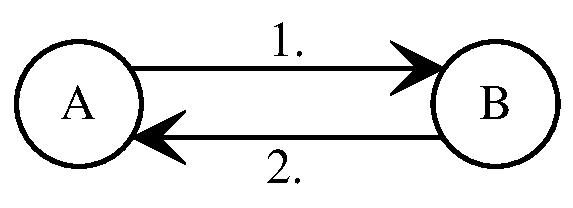
\includegraphics[width=0.5\textwidth]{pic/key_distribution-diffie-hellman}
    \caption{Общая схема взаимодействия участников в протоколе Диффи~---~Хеллмана\label{fig:key_distribution-diffie-hellman}}
\end{figure}

\begin{protocol}
    \item[(1)] Алиса выбирает случайное $2 \leq a \leq p - 1$
    \item[{}] $Alice \to \left\{ A = g ^ a \bmod p \right\} \to Bob$
    \item[(2)] Боб выбирает случайное $2 \leq b \leq p-1$
    \item[{}] Боб вычисляет сеансовый ключ $K = A ^ b \bmod p$
    \item[{}] $Bob \to \left\{ B = g ^ b \bmod p \right\} \to Alice$
    \item[(3)] Алиса вычисляет $K = B ^ a \bmod p$
\end{protocol}

Таким способом создан общий секретный сеансовый ключ $K$. За счёт случайного выбора значений $a$ и $b$ в новом сеансе будет получен новой сеансовый ключ.

Протокол обеспечивает только генерацию новых сеансовых ключей (цель G10). В отсутствие третей доверенной стороны он не обеспечивает ни аутентификацию сторон (цель G1), из-за отсутствия проходов с подтверждением владения ключом отсутствует аутентификация ключа (цель G8). Зато, так как протокол не использует длительные <<мастер>>-ключи, можно говорить о том, что он обладает свойством совершенной прямой секретности (цель G9).

Протокол можно использовать только с такими каналами связи, в которые не может вмешаться активный криптоаналитик. В противном случае протокол становится уязвим к простой <<атаке посередине>>.

\begin{figure}
    \centering
    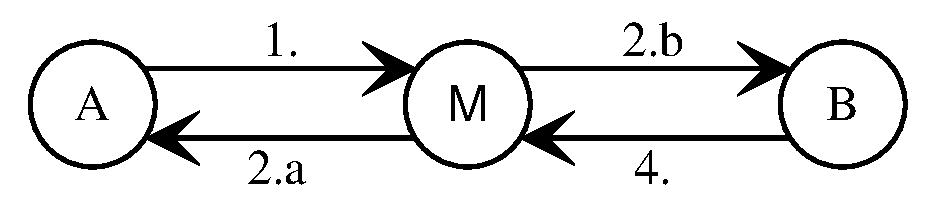
\includegraphics[width=0.67\textwidth]{pic/key_distribution-diffie-hellman-mitm}
    \caption{Схема взаимодействия участников в протоколе Диффи~---~Хеллмана в модели с активным криптоаналитиком\label{fig:key_distribution-diffie-hellman-mitm}}
\end{figure}

\begin{protocol}
    \item[(1)] Алиса выбирает случайное $2 \leq a \leq p - 1$
    \item[{}] $Alice \to \left\{ A = g ^ a \bmod p \right\} \to Mellory~(Bob)$
    \item[(2)] Меллори выбирает случайное $2 \leq m \leq p-1$
    \item[{}] Меллори вычисляет сеансовый ключ для канала с Алисой
        \[K_{AM} = A ^ m \bmod p = g ^ {am} \bmod p\]
    \item[{}] $Mellory~(Alice) \to \left\{ M = g ^ m \bmod p \right\} \to Bob$
    \item[{}] $Mellory~(Bob) \to \left\{ M = g ^ m \bmod p \right\} \to Alice$
    \item[(3)] Алиса вычисляет сеансовый ключ для канала с Меллори (думая, что Меллори это Боб)
        \[K_{AM} = M ^ a \bmod p = g ^ { am } \bmod p\]
    \item[(4)] Боб выбирает случайное $2 \leq b \leq p-1$
    \item[{}] Боб вычисляет сеансовый ключ для канала с Меллори (думая, что Меллори это Алиса)
        \[K_{BM} = M ^ b \bmod p = g ^ { bm } \bmod p\]
    \item[{}] $Bob \to \left\{ B = g ^ b \bmod p \right\} \to Mellory~(Alice)$
    \item[(5)] Меллори вычисляет сеансовый ключ для канала с Бобом
        \[K_{BM} = B ^ m \bmod p = g ^ { bm } \bmod p\]
\end{protocol}

В результате Алиса и Боб получили новые сеансовые ключи, но <<защищённый>> канал связи установили не с друг с другом, а со злоумышленником, который теперь имеет возможность ретранслировать или изменять все передаваемые сообщения между Алисой и Бобом.

Протокол Диффи~---~Хеллмана отличается от большей части протоколов распространения ключей из-за того, что не использует другие криптографические примитивы (функции шифрования, электронно-цифровой подписи или хеширования), но сам по себе является в некотором смысле криптографическим примитивом для построения более сложных протоколов. Он обеспечивает генерацию случайного числа в распределённой системе без доверенного центра. Причём ни одна из сторон не может заставить другую сторону использовать старый сессионный ключ, в отличие от, например, протокола Yahalom\index{протокол!Yahalom} из раздела~\ref{section-protocols-yahalom}.

Протокол можно изменить таким образом, чтобы вместо мультипликативной группы простого умножения использовать аддитивную группу сложения точек эллиптической кривой (см. раздел~\ref{section-math-ec-groups}). В этом случае стороны по прежнему будут выбирать некоторые случайные целые числа, но не возводить генератор-число в степень, а умножать генератор-точку на загаданное число.

\begin{protocol}
    \item[(0)] Стороны договорились о группе точек эллиптической кривой $\group{E}$, её циклической подгруппе $\group{G}$ мощности $n = \| \group{G} \|$ и генераторе $G$ группы $\group{G}$ (или хотя бы достаточно большой подгруппы группы $\group{G}$).
    \item[(1)] Алиса выбирает случайное $2 \leq a \leq n - 1$
    \item[{}] $Alice \to \left\{ A = a \times G \right\} \to Bob$
    \item[(2)] Боб выбирает случайное $2 \leq b \leq n - 1$
    \item[{}] Боб вычисляет точку $K = b \times A$
    \item[{}] $Bob \to \left\{ B = g \times G \right\} \to Alice$
    \item[(3)] Алиса вычисляет точку $K = a \times B$
\end{protocol}

В качестве нового сессионного ключа стороны могут выбрать, например, первую координату найденной точки $K$.


%\section{Протоколы с аутентификацией}

\subsection{Односторонняя аутентификация}

\section{Системы Эль-Гамаля}
\selectlanguage{russian}

\subsection[Шифрование]{Система шифрования Эль-Гамаля}

Эта система шифрования с открытым ключом опубликована Эль-Гамалем (El-Gamal) в 1985 году. Рассмотрим принципы ее построения.

Пусть имеется мультипликативная группа $\Z_p^* = \{1, 2, \dots, p-1\}$, где $p$ -- большое простое число, содержащее 1024 двоичных разряда. Существует целое число $g$, называемое примитивным элементом, который порождает все ненулевые числа группы, причем $1 < g < p-1$.

    \[ g\mod p, ~~ g^2\mod p, ~~ \dots, ~~ g^{p-1} = 1\mod p \]

Выберем целое число $x$ в интервале $1 \le x \le p-1$. Вычислим
    \[ y = g^x \mod p. \]
Известно, что в конечном поле функция $y(x)$ -- вычислительно однонаправленная.

Задачей \textbf{дискретного логарифмирования}\index{задача!дискретного логарифмирования} в мультипликативной группе $\Gr$ называется нахождение $x$ по заданным элементам $a,b \in \Gr, ~ b = a^x$. Для групп большого размера $2^{150}$--$2^{1000}$ при выборе элемента $a$ генератором группы или подгруппы большого порядка дискретный логарифм известными алгоритмами не вычислим за доступное время, все известные алгоритмы -- неполиномиальные.

Процедура шифрования криптосистемы  Эль-Гамаля состоит из следующих операций.

\begin{enumerate}
    \item \textbf{Создание пары из секретного и открытого ключей стороной $A$.}
        \begin{enumerate}
            \item $A$ выбирает простое случайное число $p$.
            \item Выбирает генератор $g$ (в программных реализациях алгоритма генератор часто выбирается малым числом, например $g = 2 \mod p$).
            \item Выбирает $x \in [1, p-1]$ с помощью генератора случайных чисел.
            \item Вычисляет $y=g^{x}\mod p$,
            \item Создает секретный и открытые ключи $\SK$ и $\PK$:
                \[ \SK = (x), ~ \PK = (p, g, y). \]
                Криптостойкость задается битовой длиной параметра $p$.
        \end{enumerate}
    \item \textbf{Шифрование на открытом ключе стороной $B$.}
        \begin{enumerate}
            \item $B$ извлекает открытый ключ $\text{PK} = (p, g, y)$ из директории стороны $A$.
            \item Сообщение представляется числом $m \in [1,p-1]$.
            \item Выбирает случайное число $r \in [1, p-1]$ и вычисляет
                \[ \begin{array}{l}
                    a = g^r \mod p, \\
                    b = m y^r \mod p.
                \end{array} \]
            \item Создает шифрованное сообщение в виде
                \[ c = (a,b) \]
                и посылает стороне $A$.
        \end{enumerate}
    \item \textbf{Расшифрование на секретном ключе стороной $A$.}
        \begin{enumerate}
            \item Используя секретный ключ $x$, $A$ вычисляет
                \[ m = \frac{b}{a^x} \mod p. \]
            \item Расшифрование корректно, так как
                \[ \begin{array}{l}
                    \frac{b}{a^x} = \frac{m y^r}{g^{rx}} = m \mod p, \\
                    m \mod p \equiv m.
                \end{array} \]
        \end{enumerate}
\end{enumerate}


\subsubsection{Пример системы}

\begin{enumerate}
    \item Генерирование параметров.
        \begin{enumerate}
            \item Выберем $p=41$.
            \item Группа $\Z_p^*$ циклическая, найдем генератор (примитивный элемент). Порядок группы
                \[ |\Z_p^*| = \phi(p) = p-1 = 40. \]
                Делители 40: 2, 4, 5, 8, 10, 20. Элемент группы является примитивным, если все его степени, соответствующие делителям порядка группы, не сравнимы с 1. Из табл. \ref{tab:elgamal-generator-search} видно, что число $g = 6$ является генератором всей группы.
                \begin{table}[h!]
                    \centering
                    \caption{Поиск генератора в циклической группе $\Z_{41}^*$. Элемент 6 -- генератор\label{tab:elgamal-generator-search}}
                    \resizebox{\textwidth}{!}{ \begin{tabular}{|c|c|c|c|c|c|c|c|c|}
                        \hline
                        \multirow{2}{*}{Элемент} & \multicolumn{7}{|c|}{Степени} & \multirow{2}{*}{Порядок элемента} \\
                        \cline{2-8}
                                & 2   & 4   & 5   & 8  & 10 & 20 & 40 & \\
                        \hline
                        2       & 4   & 16  & -9  & 10 & -1 & 1  &    & 20 \\
                        3       & 9   & -1  & -3  & 1  &    &    &    & 8 \\
                        5       & -16 & 10  & 9   & 18 & -1 & 1  &    & 20 \\
                        6       & -5  & -16 & -14 & 10 & -9 & -1 & 1  & 40 \\
                        \hline
                    \end{tabular} }
                \end{table}
            \item Выберем случайное $x = 19 \in [1, p-1]$.
            \item Вычислим
                \[ \begin{array}{ll}
                    y & = g^x \mod p = \\
                    & = 6^{19} \mod 41 = \\
                    & = 6^{1 + 2 + 4 \cdot 0 + 8 \cdot 0 + 16} \mod 41 = \\
                    & = 6^1 \cdot 6^2 \cdot 6^{4 \cdot 0} \cdot 6^{8 \cdot 0} \cdot 6^{16} \mod 41 = \\
                    & = 6 \cdot (-5) \cdot (-16)^0 \cdot 10^0 \cdot 18 \mod 41 = \\
                    & = -7 \mod 41.
                \end{array} \]
            \item Открытый и секретные ключи:
                \[ \PK = (p:41, g:6, y:-7), ~ \SK = (x:19). \]
        \end{enumerate}
    \item Шифрование.
        \begin{enumerate}
            \item Пусть сообщением является число $m = 3 \in \Z_p^*$.
            \item Выберем случайное число $r = 25 \in [1, p-1]$.
            \item Вычислим
                \[ \begin{array}{l}
                    a = g^r \mod p = 6^{25} \mod 41 = 14 \mod 41, \\
                    b = m y^r \mod p = 3 \cdot (-7)^{25} \mod 41 = -9 \mod 41.
                \end{array} \]
            \item Шифротекстом является пара чисел
                \[ c = (a:14, ~ b:-9). \]
        \end{enumerate}
    \item Расшифрование.
        \begin{enumerate}
            \item Пусть получен шифротекст
                \[ c = (a:14, ~ b:-9). \]
            \item Вычислим открытый текст как
                \[ \begin{array}{ll}
                    m & = \frac{b}{a^x} \mod p = \\
                    & = -9 \cdot (14^{-1})^{19} \mod 41 = \\
                    & = -9 \cdot 3^{19} \mod 41 = \\
                    & = -9 \cdot (-14) \mod 41 = \\
                    & = 3 \mod 41. \\
                \end{array} \]
        \end{enumerate}
\end{enumerate}


\subsection[Электронная цифровая подпись]{Электронная цифровая подпись \protect\\ Эль-Гамаля}

Криптосистема Эль-Гамаля, как и криптосистема RSA,  может быть использована для создания ЭЦП.

По-прежнему имеются два пользователя $A$ и $B$ и незащищенный канал связи между ними. Пользователь $A$  хочет подписать свое открытое сообщение $m$  для того, чтобы пользователь $B$ мог убедиться, что именно $A$ подписал сообщение.

Пусть $A$ имеет секретный ключ $\SK = (x)$, открытый ключ $\PK = (p,g,y)$ (полученные так же, как и в системе шифрования Эль-Гамаля) и хочет подписать открытое сообщение. Обозначим подпись $S(m)$.

Для создания подписи $S(m)$ пользователь $A$ выполняет следующие операции:
\begin{itemize}
    \item вычисляет значение криптографической хэш-функции  $h(m) \in [0,p-2]$, от своего открытого сообщения $m$;
    \item выбирает случайное число $r, ~ \gcd(r, p-1)=1$;
    \item используя открытый ключ, вычисляет
        \[ \begin{array}{l}
            a = g^r \mod p, \\
            b = \frac{h(m) - xa}{r} \mod (p-1); \\
        \end{array} \]
    \item создает подпись в виде двух чисел
        \[ S(m) = (a, b) \]
        и посылает сообщение с подписью $(m, S(m))$.
\end{itemize}

Получив сообщение,  $B$ осуществляет проверку подписи, выполняя следующие операции:
\begin{itemize}
    \item по известному сообщению $m$ вычисляет значение хэш-функции $h(m)$;
    \item вычисляет
        \[ \begin{array}{l}
            f_1 = g^{h(m)} \mod p, \\
            f_2 = y^a a^b \mod p; \\
        \end{array} \]
    \item сравнивает значения $f_1$ и $f_2$, если
        \[ f_1 = f_2, \]
        то подпись подлинная, в противном случае -- фальсифицированная (или случайно испорченная).
\end{itemize}

Покажем, что проверка подписи корректна. По малой теореме Ферма получаем
\[ \begin{array}{ll}
    f_1 & = g^{h(m)} \mod p = \\
    & \\
    & = g^{h(m) \mod (p-1)} \mod p; \\
\end{array} \] \[ \begin{array}{ll}
    f_2 & = y^a a^b \mod p = \\
    & = \underbrace{\left( g^x \right)^a}_{y^a} \cdot
        \underbrace{\left( g^r \mod p \right)^{\frac{h(m) - xa}{r} \mod (p-1)}}_{a^b} \mod p = \\
    & \\
    & = g^{xa \mod (p-1)} ~\cdot~ g^{h(m) - xa \mod (p-1)} \mod p = \\
    & = g^{h(m) \mod (p-1)} \mod p = \\
    & = f_1.
\end{array} \]

\subsubsection{Пример системы}

\begin{enumerate}
    \item Генерирование параметров.
        \begin{enumerate}
            \item Выберем $p=41$.
            \item Выберем генератор $g=6$ в группе $\Z_{41}^*$.
            \item Выберем случайное $x = 19 \in [1, p-1]$.%, ~ \gcd(x, p-1) = 1$.
            \item Вычислим
                \[ \begin{array}{ll}
                    y & = g^x \mod p = \\
                    & = 6^{19} \mod 41 = \\
                    & = 6^{1 + 2 + 4 \cdot 0 + 8 \cdot 0 + 16} \mod 41 = \\
                    & = 6 \cdot (-5) \cdot (-16)^0 \cdot 10^0 \cdot 18 \mod 41 = \\
                    & = -7 \mod 41. \\
                \end{array} \]
            \item Открытый и секретные ключи:
                \[ \PK = (p:41, g:6, y:-7), ~ \SK = (x:19). \]
        \end{enumerate}
    \item Подписание.
        \begin{enumerate}
            \item От сообщения $m$ вычисляется хэш $h = H(m)$. Пусть хэш $h  = 3 \in [0, p-2]$.
            \item Выберем случайное $r = 9 \in [1, p-2]$: \\
                $\gcd(r=9, p-1 = 40) = 1$.
            \item Вычислим
                \[ \begin{array}{ll}
                    a & = g^r \mod p = \\
                      & = 6^9 \mod 41 = 19 \mod 41, \\
                    b & = \frac{h - xa}{r} \mod (p-1) = \\
                      & = (3 - 19 \cdot 19) \cdot 9^{-1} \mod 40 = \\
                      & = 2 \cdot 9 \mod 40 = 18 \mod 40. \\
                \end{array} \]
            \item Подпись
                \[ s = (a:19, b:18). \]
        \end{enumerate}
    \item Проверка подписи.
        \begin{enumerate}
            \item Для полученного сообщения находится хэш $h = H(m) = 3$. Пусть полученная подпись к нему имеет вид
                \[ s = (a:19, b:18). \]
            \item Вычислим
                \[ \begin{array}{ll}
                    f_1 & = g^h \mod p = \\
                        & = 6^3 \mod 41 = 11 \mod 41, \\
                    f_2 & = y^a a^b \mod p = \\
                        & = (-7)^{19} \cdot 19^{18} \mod 41 = 11 \mod 41. \\
                \end{array} \]
            \item Проверим равенство $f_1$ и $f_2$. Подпись верна, так как
                \[ f_1 = f_2 = 11. \]
        \end{enumerate}
\end{enumerate}


\subsection[Криптостойкость]{Криптостойкость систем \protect\\ Эль-Гамаля}

Пусть дано уравнение $y=g^{x} \mod p$, требуется определить $x$ в интервале $0<x<p-1$. Задача называется \textbf{дискретным логарифмированием}\index{задача!дискретного логарифма}.

Рассмотрим возможные способы нахождения неизвестного числа $x$. Начнем с перебора различных значений $x$ из интервала $0<x<p-1$ и проверке равенства $y=g^{x} \mod p$. Число попыток в среднем равно $\frac{p}{2}$, при $p=2^{1024}$ это число равно $2^{1023}$, что на практике не осуществимо.

Другой подход предложен советским математиком Гельфондом\index{алгоритм!Гельфонда} безотносительно к криптографии. Он состоит в следующем.
Вычислим $S=\lceil\sqrt{p-1}\rceil $, где скобки означают ближайшее (сверху) целое от числа $\sqrt{p-1} $.

Представим искомое число $x$   в следующем виде

\begin{equation}
    x=x_{1} S+x_{2},
    \label{S}
\end{equation}

где $x_{1}$ и $x_{2}$ -- целые неотрицательные числа,
    \[ x_{1} \le S-1, ~ x_{2} \le S-1. \]
Такое представление является однозначным.

Вычислим и занесем в таблицу следующие $S$  чисел:
    \[ g^{0} \mod p, ~~ g^{1} \mod p, ~~ g^{2} \mod p, ~~ \dots, ~~ g^{S-1} \mod p. \]
Вычислим $g^{-S} \mod p$ и также занесем в таблицу.

\begin{center} \begin{tabular}{|l|c|c|c|c|c|c|}
    \hline
    $\lambda $ & 0 & 1 & 2 & \dots & $S-1$ & $-S$ \\
    \hline
    $g^{\lambda} \mod p$ & $g^{0}$ & $g^{1}$ & $g^{2}$ & \dots & $g^{S-1}$ & $g^{-S}$ \\
    \hline
\end{tabular} \end{center}

Для решения уравнения \ref{S} используем перебор значений $x_{1}$.
\begin{enumerate}
    \item  Предположим, что $x_{1} = 0$. Тогда $x = x_{2}$.  Если число $y = g^{x_{2}} \mod p$ содержится в таблице, то  находим его и выдаем результат: $x=x_{2} $. Задача решена. В противном случае переходим к пункту 2.
    \item  Предположим, что $x_{1} =1$. Тогда $x=S+x_{2} $ и $y=g^{S+x_{2}} \mod p$. Вычисляем $yg^{-S} \mod p=g^{x_{2}} \mod p$. Задача сведена к предыдущей: если $g^{x_{2} } \mod p$ содержится в таблице, то в таблице находим число $x_{2} $ и выдаем результат $x$: $x=S+x_{2} $.
    \item  Предположим, что $x_{1} =2$. Тогда $x=2S+x_{2} $ и $y=g^{2S+x_{2} } \mod p$. Если число $yg^{-2S} \mod p=g^{x_{2} } \mod p$ содержится в таблице, то находим число $x_{2}$ и выдаем результат: $x = 2S + x_{2}$.
     \item  Пробегая все возможные значения, доберемся, в худшем случае, до $x_{1} =S-1$. Тогда $x=(S-1)S+x_{2} $ и $y = g^{(S-1)S+x_{2} } \mod p$. Если число $yg^{-(S-1)S} \mod p=g^{x_{2}} \mod p$ содержится в таблице, то  находим его и выдаем результат: $x=(S-1)S+x_{2}$.
\end{enumerate}

Легко проверить, что с помощью построенной таблицы мы проверили все возможные значения $x$. Максимальное число умножений равно $2S \approx 2\sqrt{p-1} =2\times 2^{512} $, что для практики очень велико.  Тем самым проблему достаточной криптостойкости этой системы можно было бы считать решенной. Однако это не верно, так как числа $p-1$ являются составными. Если  $p-1$ можно разложить на маленькие множители, то криптоаналитик может применить процедуру, подобную процедуре Гельфонда, по взаимно простым делителям  $p-1$  и найти секрет. Пусть  $p-1=st$. Тогда элемент $g^s$ образует подгруппу порядка $t$ и наоборот. Теперь, решая уравнение $y^s=(g^s)^a\mod p$, находим вычет $x=a\mod t$. Поступая аналогично, находим $x=b\mod s$ и по Китайской теореме об остатках находим $x$.

Несколько позже подобный метод ускоренного решения уравнения \ref{S} был предложен Шенксом (Shanks)и Хеллманом (Hellman). В англоязычной технической литературе он получил название алгоритма Шенкcа.

Пусть $k = \lceil \log_2 p \rceil$ -- битовая длина числа $p$. Алгоритм Гельфонда имеет  экспоненциальную сложность (число двоичных операций)
    \[ O(\sqrt{p}) = O(e^{\frac{1}{2} \frac{1}{\log_2 e} k}). \]

Наилучшие из известных алгоритмов решения задачи дискретного логарифма имеют экспоненциальную сложность порядка
    \[ O(e^{\sqrt{k}}). \]


\subsection{Взаимная аутентификация шифрованием}
\selectlanguage{russian}

К протоколам взаимной аутентификации принадлежит семейство протоколов, разработанных Т. Мацумото (T. Matsumoto), И. Такашима (Y. Takashima) и Х. Имаи (H. Imai) и названных по первым буквам фамилий авторов -- \textbf{протокол MTI}\index{протокол!MTI}.

Здесь к открытым данным относятся
    \[ p, ~~ g, ~~ \PK_A = g^a \mod p, ~~ \PK_B = g^b \mod p. \]
Каждый пользователь $A$ и $B$ обладает парой долговременных ключей для \emph{схемы шифрования с открытым ключом}: закрытый ключ расшифрования $\SK$ и открытый ключ шифрования  $\PK$.
\[ \begin{array}{ll}
    A: & ~ \SK_A = a, ~~ \PK_A = g^a \mod p, \\
    B: & ~ \SK_B = b, ~~ \PK_B = g^b \mod p. \\
\end{array} \]

\textbf{Протокол MTI}:
\begin{enumerate}
    \item Сторона $A$ генерирует случайное число $x, ~ 2\leq x\leq p-1$, создает и отправляет $B$ сообщение:
        \[ A \rightarrow B: ~ g^x \mod p. \]
    \item Сторона $B$ генерирует случайное число $y, ~ 2\leq y\leq p-1$, создает и отправляет $A$ сообщение:
        \[ A \leftarrow B: ~ g^y \mod p. \]
    \item Сторона $A$, используя открытые данные и полученное сообщение, создает сеансовый ключ:
        \[ K_A = (g^b)^x \cdot (g^y)^a = g^{bx+ay} \mod p. \]
    \item Сторона $B$, используя открытые данные и полученное сообщение, создает сеансовый ключ:
        \[ K_B = (g^x)^b \cdot (g^a)^y = g^{bx+ay} \mod p. \]
        Сеансовые ключи обоих сторон совпадают:
        \[ K_{A} =K_{B} = K. \]
\end{enumerate}

В описанном протоколе происходит взаимная аутентификация сторон как и в протоколе Эль-Гамаля\index{криптосистема!Эль-Гамаля}: открытые ключи сторон незаметно подменить невозможно. Наблюдая сообщения протокола, вычислить $g^{bx+ay}$ можно, только если известны значения $a,x$ или $b,y$, что представляет собой задачу дискретного логарифма, трудную в вычислительном смысле в настоящее время.


\subsection{Протокол Station-to-Station}\label{section-protocols-sts}\index{протокол!Station-to-Station|(}
\selectlanguage{russian}

Протокол STS (\langen{Station-to-Station},~\cite{Diffie:Oorschot:Wiener:1992})\index{протокол!Station-to-Station} предназначен для систем мобильной связи. Он использует идеи протокола Диффи~---~Хеллмана\index{протокол!Диффи~---~Хеллмана} и криптосистемы RSA\index{криптосистема!RSA}. Особенностью протокола является использование механизма электронной подписи\index{электронная подпись} для взаимной аутентификации сторон\index{аутентификация!взаимная}.

Предварительно стороны договорились об общих параметрах системы $p$ и $g$, где $p$ -- большое простое число, а $g$ -- примитивный элемент поля $\Z_p^*$.

Каждая из сторон $A$ и $B$ обладает долговременной парой ключей: закрытым ключом для расшифрования и создания электронной подписи $K_{\text{private}}$ и открытым ключом для шифрования и проверки подписи $K_{\text{public}}$.

\[\begin{array}{ll}
    A: K_{A,\text{private}}, K_{A,\text{public}}: \forall M : & \text{Verify}_A ( M, S_A( M ) ) = true, \\
                                                & D_A ( E_A( M ) ) = M, \\
    B: K_{B,\text{private}}, K_{B,\text{public}}: \forall M : & \text{Verify}_B ( M, S_B( M ) ) = true, \\
                                                & D_B ( E_B( M ) ) = M. \\
\end{array}\]

Где $\text{Verify}_A(\dots)$ это функция проверки электронной подписи на открытом ключе $K_{A, \text{public}}$, а $D_A$ -- функция расшифрования с использованием закрытого ключа $K_{A, \text{private}}$.

Протокол состоит из четырёх проходов, три из которых включают передачу сообщений (рис.~\ref{fig:key_distribution-sts}, \cite{Cheremushkin:2009}).

\begin{figure}
    \centering
    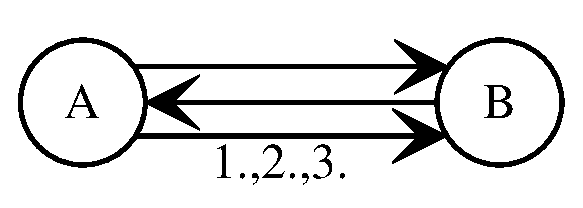
\includegraphics[width=0.5\textwidth]{pic/key_distribution-sts}
    \caption{Взаимодействие участников в протоколе STS\label{fig:key_distribution-sts}}
\end{figure}

\begin{protocol}
    \item[(1)] Алиса выбирает случайное число $R_A: 2 \leq R_A \leq p-1$.
    \item[{}] $Alice \to \left\{ A, m_A = g^{R_A} \bmod p \right\} \to Bob$

    \item[(2)] Боб выбирает случайное число $R_B: 2 \leq R_B \leq p-1$.
    \item[{}] Боб вычисляет сессионный ключ $K = m_A^{R_B} \bmod p$.
    \item[{}] $Bob \to \left\{ B, A, m_B = g^{R_B} \bmod p, E_K( S_B ( m_A, m_B )) \right\} \to Alice$

    \item[(3)] Алиса вычисляет сессионный ключ $K = m_B^{R_A} \bmod p$.
    \item[{}] Алиса проверяет подпись в сообщении $E_K( S_B ( m_A, m_B ))$.
    \item[{}] $Alice \to \left\{ A, B, E_K( S_A ( m_A, m_B ) ) \right\} \to Bob$

    \item[(4)] Боб проверяет подпись в сообщении $E_K( S_A ( m_A, m_B ))$.
\end{protocol}

Протокол обеспечивает гарантию формирования новых ключей (G10), но не совершенную прямую секретность (G9).

Как показала атака Лоу 1996 года (\cite{Lowe:1996}, рис.~\ref{fig:key_distribution-sts-attack}), протокол не может гарантировать аутентификацию субъектов (цель G1), ключей (G7) и подтверждение владения сессионным ключом (G8). Хотя злоумышленник не может получить доступ к новому сессионному ключу, если протокол использовать только для аутентификации субъектов, Алиса может принять злоумышленника за Боба.

\begin{figure}
    \centering
    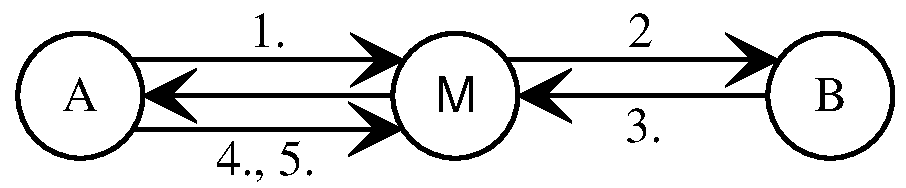
\includegraphics[width=0.67\textwidth]{pic/key_distribution-sts-attack}
    \caption{Схема взаимодействия участников в протоколе STS при атаке Лоу\label{fig:key_distribution-sts-attack}}
\end{figure}

\begin{protocol}
    \item[(1)] Алиса выбирает случайное число $R_A: 2 \leq R_A \leq p-1$.
    \item[{}] $Alice \to \left\{ A, m_A = g^{R_A} \bmod p \right\} \to Mellory~(Bob)$

    \item[(2)] $Mellory~(Alice) \to \left\{ M, m_A \right\} \to Bob$

    \item[(3)] Боб выбирает случайное число $R_B: 2 \leq R_B \leq p-1$ и вычисляет $m_B = g^{R_B} \bmod p$, а также сессионный ключ $K = m_A^{R_B} \bmod p$.
    \item[{}] $Bob \to \left\{ B, M, m_B, E_K( S_B ( m_A, m_B )) \right\} \to Mellory$

    \item[(4)] $Mellory~(Bob) \to \left\{ B, A, m_B, E_K( S_B ( m_A, m_B )) \right\} \to Alice$

    \item[(5)] Алиса вычисляет сессионный ключ $K = m_B^{R_A} \bmod p$.
    \item[{}] Алиса проверяет подпись в сообщении $E_K( S_B ( m_A, m_B ))$.
    \item[{}] $Alice \to \left\{ A, B, E_K( S_A ( m_A, m_B ) ) \right\} \to Mellory~(Bob)$
\end{protocol}

После успешного завершения протокола Алиса уверена, что общается с Бобом.

Как и все остальные <<криптосистемы-протоколы>>, протокол Station-to-Station основывается на некотором внешнем источнике информации об открытых ключах участников, не подвергая сомнению корректность и надёжность этого источника. Что, в общем случае, неверно. Если информацию о ключах участников нужно получать извне при каждом сеансе протокола (например, если участников много, и запомнить ключи всех возможности нет), то канал получения открытых ключей будет основной целью активного криптоаналитика для рассмотренных протоколов. Как от этого защититься с использованием примитивов асимметричной криптографии -- в разделе~\ref{section-protocols-asymmetric}.

\index{протокол!Station-to-Station|)}

\subsection{Схема Жиро}\label{section-girault-scheme}\index{схема!Жиро|(}
\selectlanguage{russian}

В схеме Жиро (\langfr{Marc Girault},~\cite{Girault:1990, Girault:1991}) надёжность строится на стойкости криптосистемы RSA (сложности факторизации больших чисел и вычисления дискретного корня).

Предварительно:
\begin{itemize}
    \item Доверенный центр (Трент, $T$):
    \begin{itemize}
        \item выбирает общий модуль $n = p \times q$, где $p$ и $q$ -- большие простые числа;
        \item выбирает пару из закрытого и открытого ключей $K_{T, \text{public}}: (e, n)$ и $K_{T, \text{private}}: (d, n)$;
        \item выбирает элемент $g$ поля $\mathbb{Z}_n^{\times}$ максимального порядка;
        \item публикует в общедоступном месте параметры схемы $n$, $e$ и $g$.
    \end{itemize}
    \item Каждый из легальных участников:
    \begin{itemize}
        \item выбирает себе закрытый ключ $s_i$ и идентификатор $I_i$;
        \item вычисляет и отправляет доверенному центру $v_i = g^{-s_i} \bmod n$;
        \item используя протокол аутентификации сторон (см. ниже) легальный участник доказывает доверенному центру, что владеет закрытым ключом, не раскрывая его значение;
        \item получает от доверенного центр свой открытый ключ:
            \[ P_i = (v_i - I_i)^d = (g^{-s_i} - I_i)^d \mod n; \]
    \end{itemize}
    В результате для каждого участника, например, Алисы, которая владеет $P_A, I_A, s_a$ будет выполняться утверждение:
        \[ P_A^e + I_A = g^{-s_A} \mod n. \]
\end{itemize}

Протокол аутентификации сторон в общем случае выглядит следующим образом (рис.~\ref{fig:key_distribution-girault-auth}).

\begin{figure}
    \centering
    \includegraphics[width=0.5\textwidth]{pic/key_distribution-girault-auth}
    \caption{Взаимодействия участников в протоколе идентификации Жиро\label{fig:key_distribution-girault-auth}}
\end{figure}

\begin{protocol}
    \item[(1)] Алиса выбирает случайное $R_A$.
    \item[{}] $Alice \to \left\{ I_A, P_A, t = g^{R_A} \right\} \to Bob$
    \item[(2)] Боб выбирает случайное $R_B$.
    \item[{}] $Bob \to \left\{ R_B \right\} \to Alice$
    \item[(3)] $Alice \to \left\{ y = R_A + s_A \times R_B \right\} \to Bob$
    \item[(4)] Боб вычисляет $v_A = P_A^e + I_A$;
    \item[{}] Боб проверяет, что $g^ y v_A^{R_B} = t$.
\end{protocol}

Протокол генерации сессионного ключа, либо просто \emph{схема Жиро}, как и другие схемы, состоит из проходов обмена открытой информацией и вычисления ключа (рис.~\ref{fig:key_distribution-girault-scheme}).

\begin{figure}
    \centering
    \includegraphics[width=0.5\textwidth]{pic/key_distribution-girault-scheme}
    \caption{Взаимодействие участников в схеме Жиро\label{fig:key_distribution-girault-scheme}}
\end{figure}

\begin{protocol}
    \item[(1)] $Alice \to \left\{ P_A, I_A \right\} \to Bob$
    \item[(2)] Боб вычисляет $K_{BA} = (P_A^e + I_A)^{s_B} \bmod n$.
    \item[{}] $Bob \to \left\{ P_B, I_B \right\} \to Alice$
    \item[(3)] Алиса вычисляет $K_{AB} = (P_B^e + I_B)^{s_A} \bmod n$.
\end{protocol}

В результате работы схемы стороны сгенерировали одинаковый общий сеансовый ключ.
\[ K_{AB} = (P_A^e + I_A)^{s_B} = (g^{-s_A})^{s_B} = g^{-s_As_B} \mod n; \]
\[ K_{BA} = (P_B^e + I_B)^{s_A} = (g^{-s_B})^{s_A} = g^{-s_As_B} \mod n; \]
            \[ K = K_{AB} = K_{BA} = g^{-s_As_B} \mod n. \]

Схема обеспечивает аутентификацию ключа (цель G7), так как только легальные пользователи смогут вычислить корректное значение общего сессионного ключа.

\index{схема!Жиро|)}

\subsection{Схема Блома}\index{схема!Блома}
\selectlanguage{russian}

Рассмотрим распределение ключей по \emph{схеме Блома} (Rolf Blom,~\cite{Blom:1984, Blom:1985}), в котором каждые два пользователя из общего числа $N$ пользователей могут создать общий секретный ключ, причём секретные ключи каждой пары различны. Данная схема используется в протоколе HDCP\index{протокол!HDCP} (\langen{High-bandwidth Digital Content Protection}) для предотвращения копирования высококачественного видеосигнала.

На этапе инициализации доверенный центр выбирает симметричную матрицу $D_{m,m}$ над конечным полем $\GF p$. Для присоединения к сети распространения ключей новый участник либо самостоятельно, либо с помощью доверенного центра выбирает новый открытый ключ (идентификатор) $I$, представляющий собой вектор длины $k$ над $\GF p$. Доверенный центр вычисляет для нового участника закрытый ключ $K$:

\begin{equation}
	K = D_{m,m} I.
	\label{eq:blom_center_matrix}
\end{equation}

Симметричность матрицы $D_{m,m}$ доверенного центра позволяет любым двум участникам сети создать общий сеансовый ключ. Пусть Алиса и Боб -- легальные пользователи сети, то есть они обладают открытыми ключами $I_A$ и $I_B$ соответственно, а их закрытые ключи $K_A$ и $K_B$ были вычислены одним и тем же доверенным центром по формуле~\ref{eq:blom_center_matrix}. Тогда протокол выработки общего секретного ключа выглядит следующим образом.

\begin{enumerate}
	\item Алиса отправляет Бобу свой открытый ключ $I_A$.
	\item Боб отправляет Алисе свой открытый ключ $I_B$.
	\item Алиса вычисляет значение $s_{AB} = K^t_A I_B = I^t_A D_{m,m} I_B$.
	\item Боб вычисляет значение $s_{BA} = K^t_B I_A = I^t_B D_{m,m} I_A$.
\end{enumerate}

Из симметричности матрицы $D_{m,m}$ следует, что значения $s_{AB}$ и $s_{BA}$ совпадут, они же и будут являться общим секретным ключом для Алисы и Боба. Этот секретный ключ будет свой для каждой пары легальных пользователей сети.

Присоединение новых участников к схеме строго контролируется доверенным центром, что позволяет защитить сеть от нелегальных пользователей. Надёжность данной схемы основывается на невозможности восстановить исходную матрицу. Однако для восстановления матрицы доверенного центра размера $m \times m$ необходимо и достаточно всего $m$ пар линейно независимых открытых и закрытых ключей. В 2010 году компания Intel, которая является <<доверенным центром>> для пользователей системы защиты HDCP, подтвердила, что криптоаналитикам удалось найти секретную матрицу (точнее, аналогичную ей), используемую для генерации ключей в упомянутой системе предотвращения копирования высококачественного видеосигнала.



\section{Квантовые протоколы}\index{протокол!квантовые|(}
\selectlanguage{russian}

\input{bb84}

\subsection{Протокол B92 (BB92)}\index{протокол!B92|(}\index{протокол!BB92|(}
\selectlanguage{russian}

В 1992 году один из авторов протокола BB84 Чарльз Беннетт выдвинул идею (\cite{Bennett:1992}), что участникам не обязательно использовать четыре разных варианта поляризации, а достаточно двух, но неортогональных. Например, $0^{\circ}$ (<<$\to$>>) и $45^{\circ}$ (<<$\nearrow$>>). Протокол получил названия B92 и BB92.

Для каждого бита выполняется следующее.

\begin{protocol}
    \item[(1)] Алиса поляризует фотон в зависимости от бита $b_i$ и передаёт его по квантовому каналу связи Бобу:
        \begin{itemize}
            \item для $b_i=0$ поляризует под $0^{\circ}$ (<<$\to$>>);
            \item для $b_i=1$ поляризует под $45^{\circ}$ (<<$\nearrow$>>).
        \end{itemize}
    \item[(2)] Боб случайным образом выбирает один из двух базисов: $90^{\circ}$ (<<$\uparrow$>>) или $135^{\circ}$ (<<$\nwarrow$>>), и пробует детектировать фотон. Если получилось, то он делает вывод о выбранной Алисой поляризации фотона и бите $b_i$:
        \begin{itemize}
            \item если детектировал на $135^{\circ}$ (<<$\nwarrow$>>), значит Алиса выбрала поляризацию $0^{\circ}$ (<<$\to$>>) и $b_i=0$;
            \item если детектировал на $90^{\circ}$ (<<$\uparrow$>>), значит Алиса выбрала поляризацию $45^{\circ}$ (<<$\nearrow$>>) и $b_i=1$.
        \end{itemize}
    \item[{}] Боб по открытому классическому каналу связи сообщает Алисе, получилось детектировать фотон или нет. Если да, то бит принимается участниками за переданный.
\end{protocol}

\begin{table}
    \centering
    \begin{tabular}{|l|c|c|c|c|c|c|c|c|}
        \hline
        \parbox[c][1cm][c]{2,8cm}{биты Алисы} & 0 & 0 & 0 & 0 & 1 & 1 & 1 & 1 \\
        \hline
        \parbox[c][1cm][c]{2,8cm}{поляризация \\ фотона} & $\to$ & $\to$ & $\to$ & $\to$ & $\nearrow$ & $\nearrow$ & $\nearrow$ & $\nearrow$ \\
        \hline
        \parbox[c][1cm][c]{2,8cm}{поляризация \\ детектора Боба} & $\nwarrow$ & $\uparrow$ & $\nwarrow$ & $\uparrow$ & $\nwarrow$ & $\uparrow$ & $\nwarrow$ & $\uparrow$ \\
        \hline
        \parbox[c][1cm][c]{2,8cm}{вероятность детектирования} & $\frac{1}{2}$ & 0 & $\frac{1}{2}$ & 0 & 0 & $\frac{1}{2}$ & 0 & $\frac{1}{2}$ \\
        \hline
        \parbox[c][1cm][c]{2,8cm}{удалось или нет детектировать} & да & нет & нет & нет & нет & да & нет &  нет \\
        \hline
        \parbox[c][1cm][c]{2,8cm}{принятые Бобом биты} & 0 & - & - & - & - & 1 & - & - \\
        \hline
    \end{tabular}
    \caption{Пример сеансов протокола B92 / BB92. По итогам передачи 8 фотонов от Алисы Боб сумел детектировать 2 фотона, что позволило передать от Алисы к Бобу 2 бита информации}
    \label{tab:b92}
\end{table}

Если Боб выбрал поляризацию, ортогональную оригинальной, то он со 100\% вероятностью не зарегистрирует фотон. Если же поляризация неортогональна оригинальной, то с вероятностью 50\% Боб сумеет зарегистрировать фотон на детекторе. Таким образом, если Боб зарегистрировал фотон, то он будет точно знать, какой бит передавала Алиса. Если же не зарегистрировал, то это трактуется, как стирание.

Пример сеансов протоколов передачи приведён в таблице~\ref{tab:b92}.

В среднем для передачи одного бита информации Алисе и Бобу потребуется провести 4 итерации протокола. Это в два раза больше, чем в протоколе BB84\index{протокол!BB84}.

\index{протокол!B92|)}\index{протокол!BB92|)}


\subsection{Общие недостатки квантовых протоколов}
Подводя итоги, можно сказать, что квантовые протоколы распределения ключей (а именно ими пока что и ограничивается вся известная на сегодняшний день <<квантовая криптография>>) обладают как определёнными преимуществами, так и фатальными недостатками, затрудняющими их использование (и ставящими под вопрос саму эту необходимость).

\begin{itemize}
	\item Любые квантовые протоколы (как и вообще любые квантовые вычисления) требуют оригинального дорогостоящего оборудования, которое пока что нельзя сделать частью commodity-устройств или обычного сотового телефона.
	\item Квантовые каналы связи -- это всегда физические каналы связи. У них существует максимальная длина канала и определённый уровень ошибок. Для квантовых каналов (на сегодняшний день) не придумали <<повторителей>>, которые позволили бы увеличить длину безусловно квантовой передачи данных.
	\item Ни один квантовый протокол (на сегодняшний день) не может обходиться без дополнительного классического канала связи. Для такого связи требуются как минимум такой же уровень защиты, как и при использовании, например, криптографии с открытым ключом.
	\item Для всех протоколов особую проблему представляет не только доказательство корректности (что является весьма нетривиальным делом в случае наличия <<добросовестных>> помех), но и инженерная задача по реализации протокола в <<железе>>. В качестве краткой иллюстрации, например, не существует простого способа создать \emph{ровно один} фотон. Недогенерация фотонов приводит, очевидно, к ошибкам передачи, а генерация дубля в том же временном слоте -- к возможности его перехвата злоумышленником без создания помех в канале.
\end{itemize}

\index{протокол!квантовые|)}


